\documentclass[12pt,a4paper,oneside]{report}

% --- Engine Detection and Font Selection ---
\usepackage{ifxetex,ifluatex}
\ifxetex
  \usepackage{fontspec}
  \setmainfont{Times New Roman}
\else\ifluatex
  \usepackage{fontspec}
  \setmainfont{Times New Roman}
\else
  \usepackage[utf8]{inputenc}
  \usepackage[T1]{fontenc}
  \usepackage{mathptmx} % Times New Roman compatible font for pdfLaTeX
\fi\fi

% --- Page Geometry (RBU Guidelines: Left 1.5 in; Right, Top, Bottom 1.0 in) ---
\usepackage[a4paper,left=1.5in,right=1.0in,top=1.0in,bottom=1.0in]{geometry}

% --- Spacing and Typography ---
\usepackage{setspace}
\onehalfspacing
\setlength{\parskip}{6pt}
\setlength{\parindent}{0pt}

% --- Packages ---
\usepackage{graphicx}
\usepackage{amsmath,amssymb}
\usepackage{booktabs}
\usepackage{tabularx}
\usepackage{array}
\usepackage{caption}
\usepackage{subcaption}
\usepackage{float}
\usepackage{xcolor}
\usepackage{titlesec}
\usepackage{fancyhdr}
\usepackage{hyperref}
\usepackage{url}
\usepackage{cite}
\usepackage{enumitem}
\usepackage{microtype}

% --- Hyperlink Setup ---
\hypersetup{
    colorlinks=true,
    linkcolor=black,
    citecolor=black,
    urlcolor=blue,
    pdftitle={Explainable Federated Learning for Healthcare IoT Applications},
    pdfauthor={Vinamra Chandak, Devyani Gadde, Radha Singh}
}

% --- Header and Footer (Bottom-Centred Page Numbers) ---
\pagestyle{fancy}
\fancyhf{}
\fancyfoot[C]{\fontsize{12pt}{14pt}\selectfont\thepage}
\renewcommand{\headrulewidth}{0pt}
\renewcommand{\footrulewidth}{0pt}
\fancypagestyle{plain}{
    \fancyhf{}
    \fancyfoot[C]{\fontsize{12pt}{14pt}\selectfont\thepage}
    \renewcommand{\headrulewidth}{0pt}
}

% --- Headings Formatting (RBU Guidelines) ---
% Chapter: 16pt, Bold, Uppercase
\titleformat{\chapter}[display]
  {\normalfont\fontsize{16pt}{20pt}\bfseries}
  {\chaptertitlename\ \thechapter}{10pt}{\fontsize{16pt}{20pt}\bfseries}
\titlespacing*{\chapter}{0pt}{-10pt}{20pt}

% Section: 14pt, Bold
\titleformat{\section}
  {\normalfont\fontsize{14pt}{18pt}\bfseries}
  {\thesection}{1em}{}
\titlespacing*{\section}{0pt}{14pt}{6pt}

% Subsection: 12pt, Bold
\titleformat{\subsection}
  {\normalfont\fontsize{12pt}{16pt}\bfseries}
  {\thesubsection}{1em}{}
\titlespacing*{\subsection}{0pt}{10pt}{4pt}

\begin{document}

% ==============================================================================
% 1. COVER PAGE (No Page Number)
% ==============================================================================
\begin{titlepage}
\thispagestyle{empty}
\centering
{\fontsize{18pt}{22pt}\bfseries\selectfont RAMDEOBABA UNIVERSITY}\\[0.4em]
{\fontsize{14pt}{18pt}\bfseries\selectfont SCHOOL OF COMPUTER SCIENCE AND ENGINEERING}\\[1.8em]


\includegraphics[width=1.4in]{figures/rbu_logo.png}\\[1.5em]

{\fontsize{14pt}{18pt}\bfseries\selectfont B. TECH PROJECT REPORT}\\[0.5em]
{\fontsize{12pt}{16pt}\bfseries\selectfont B.Tech. in Computer Science and Engineering}\\[0.4em]
{\fontsize{12pt}{16pt}\bfseries\selectfont Idea Lab}\\[1.2em]

{\fontsize{12pt}{16pt}\selectfont ON}\\[1.2em]

{\fontsize{16pt}{22pt}\bfseries\selectfont Explainable Federated Learning for Healthcare IoT Applications}\\[2.2em]

{\fontsize{12pt}{16pt}\selectfont Submitted by}\\[0.8em]
{\fontsize{12pt}{16pt}\bfseries\selectfont
\begin{tabular}{ll}
Vinamra Chandak & (Roll No. A9-46) \\
Devyani Gadde   & (Roll No. A9-51) \\
Radha Singh     & (Roll No. A9-56)
\end{tabular}}\\[1.8em]

{\fontsize{12pt}{16pt}\selectfont Under the Guidance of}\\[0.4em]
{\fontsize{13pt}{18pt}\bfseries\selectfont Prof./Dr. Gunjan Keswani}\\[0.2em]
{\fontsize{11pt}{15pt}\selectfont Project Guide}\\[1.8em]

{\fontsize{12pt}{16pt}\bfseries\selectfont Academic Year: 2026 -- 2027}\par
\end{titlepage}

% Continuous Page Numbering from Page 1 to End
\pagenumbering{arabic}
\setcounter{page}{1}

% ==============================================================================
% 2. CERTIFICATE
% ==============================================================================
\clearpage
\begin{center}
{\fontsize{14pt}{18pt}\bfseries\selectfont RAMDEOBABA UNIVERSITY, NAGPUR}\\[0.3em]
{\fontsize{12pt}{16pt}\bfseries\selectfont Department of Computer Science and Engineering}\\[1.5em]
{\fontsize{14pt}{18pt}\bfseries\selectfont \underline{CERTIFICATE}}\\[2.0em]
\end{center}

\begin{spacing}{1.5}
This is to certify that the Project Report on \textbf{``Explainable Federated Learning for Healthcare IoT Applications''} is a bonafide work of \textbf{Vinamra Chandak (A9-46), Devyani Gadde (A9-51), and Radha Singh (A9-56)}, submitted to Ramdeobaba University, Nagpur in partial fulfilment of the requirements for the award of the Degree of Bachelor of Technology (B.Tech) in Computer Science and Engineering. It has been carried out at the Department of Computer Science and Engineering, Ramdeobaba University, Nagpur during the academic year 2026--2027.
\end{spacing}

\vspace{3.5em}

\noindent
\begin{tabularx}{\textwidth}{Xr}
\textbf{Date:} \hspace{2cm} & \textbf{Place:} Nagpur
\end{tabularx}

\vspace{4.0em}

\noindent
\begin{minipage}[t]{0.48\textwidth}
\textbf{Gunjan Keswani}\\
Project Guide\\
Department of CSE\\
Ramdeobaba University, Nagpur
\end{minipage}
\hfill
\begin{minipage}[t]{0.48\textwidth}
\raggedleft
\textbf{Associate Head}\\
Department of CSE\\
Ramdeobaba University, Nagpur
\end{minipage}

\vspace{5.0em}
\begin{center}
\textbf{Dr. P. D. Adane}\\
Dean, School of Computer Science and Engineering\\
Ramdeobaba University, Nagpur
\end{center}

% ==============================================================================
% 3. STUDENT DECLARATION
% ==============================================================================
\clearpage
\begin{center}
{\fontsize{14pt}{18pt}\bfseries\selectfont STUDENT DECLARATION}\\[2.0em]
\end{center}

\begin{spacing}{1.5}
We hereby declare that the project report entitled \textbf{``Explainable Federated Learning for Healthcare IoT Applications''} is submitted as part of the requirements for the B.Tech programme at Ramdeobaba University, Nagpur.

The work presented in this report is prepared by the undersigned students under the guidance of the project supervisor, \textbf{Prof./Dr. Gunjan Keswani}. All external sources, datasets, software tools, architectures, figures, and technical materials used in the project have been appropriately cited and acknowledged. The empirical results and numerical evaluations included in this report represent actual software-based experimental findings executed on decentralized edge nodes.
\end{spacing}

\vspace{4.0em}

\noindent
\begin{tabularx}{\textwidth}{l X r}
\textbf{Vinamra Chandak} & & Roll No. A9-46 \\[2.5em]
\textbf{Devyani Gadde} & & Roll No. A9-51 \\[2.5em]
\textbf{Radha Singh} & & Roll No. A9-56 \\
\end{tabularx}

% ==============================================================================
% 4. APPROVAL SHEET
% ==============================================================================
\clearpage
\begin{center}
{\fontsize{14pt}{18pt}\bfseries\selectfont APPROVAL SHEET}\\[2.0em]
\end{center}

\begin{spacing}{1.5}
This report entitled \textbf{``Explainable Federated Learning for Healthcare IoT Applications''} by \textbf{Vinamra Chandak, Devyani Gadde, and Radha Singh} is approved for the degree of Bachelor of Technology (B.Tech) in Computer Science and Engineering.
\end{spacing}

\vspace{5.0em}

\noindent
\begin{minipage}[t]{0.48\textwidth}
\textbf{Gunjan Keswani}\\
Project Guide\\
Department of CSE\\
Ramdeobaba University, Nagpur
\end{minipage}
\hfill
\begin{minipage}[t]{0.48\textwidth}
\raggedleft
\textbf{External Examiner}\\
(Name and Signature)\\
Ramdeobaba University, Nagpur
\end{minipage}

\vspace{5.0em}
\begin{center}
\textbf{Dr. P. D. Adane}\\
Dean, School of Computer Science and Engineering\\
Ramdeobaba University, Nagpur
\end{center}

% ==============================================================================
% 5. ACKNOWLEDGEMENT
% ==============================================================================
\clearpage
\begin{center}
{\fontsize{14pt}{18pt}\bfseries\selectfont ACKNOWLEDGEMENT}\\[2.0em]
\end{center}

\begin{spacing}{1.5}
We express our sincere gratitude to \textbf{Ramdeobaba University} and the \textbf{School of Computer Science and Engineering} for providing the academic environment, computational infrastructure, and IDEA Lab facilities required to complete this project.

We are deeply grateful to our project guide, \textbf{Prof./Dr. Gunjan Keswani}, for continuous guidance, insightful technical suggestions, and constructive feedback throughout the system design, implementation, and evaluation phases. We also extend our gratitude to the Project In-Charge, the Associate Head, and \textbf{Dr. P. D. Adane}, Dean, School of Computer Science and Engineering, for their encouragement and administrative support.

We acknowledge the support of our classmates, laboratory technical staff, friends, and family members who contributed directly or indirectly to the successful completion of this work.
\end{spacing}

\vspace{3.5em}
\noindent
\textbf{Vinamra Chandak}\\
\textbf{Devyani Gadde}\\
\textbf{Radha Singh}

% ==============================================================================
% 6. ABSTRACT & KEYWORDS
% ==============================================================================
\clearpage
\begin{center}
{\fontsize{14pt}{18pt}\bfseries\selectfont ABSTRACT}\\[1.5em]
\end{center}

\begin{spacing}{1.5}
Internet of Medical Things (IoMT) devices and point-of-care telemetry systems generate continuous streams of high-dimensional physiological indicators essential for clinical decision support. However, centralizing sensitive patient telemetry into cloud repositories violates privacy regulations, including HIPAA, GDPR, and the Digital Personal Data Protection (DPDP) Act, while introducing communication latency and single points of failure. Conversely, isolated models trained within single hospital silos exhibit poor generalizability across heterogeneous patient cohorts. Furthermore, deep clinical models often operate as opaque black boxes, preventing clinical adoption due to a lack of interpretable feature attribution.

This project proposes, implements, and evaluates the \textbf{XFL-IoMT Clinical Decision Gateway}, a privacy-preserving edge architecture coupling Federated Learning (FL) via Federated Averaging (FedAvg) over gRPC with localized Explainable Artificial Intelligence (XAI) using Shapley Additive exPlanations (SHAP). The system enforces physical data locality: raw patient records and SHAP reference background cohorts are confined within independent edge hospital containers (\texttt{hospital\_a.db} and \texttt{hospital\_b.db}). The edge microservice supports dynamic dual-model execution between a baseline Logistic Regression model and a non-linear PyTorch Multi-Layer Perceptron (CardiacMLP). On-premise SHAP attribution is computed against local demographic reference cohorts ($N=50$), producing exact directional risk shifts without raw data egress.

Empirical evaluation on an independent held-out cardiovascular test set ($N=150$) demonstrates that global FedAvg achieves an accuracy of $61.33\%$, an F1-score of $0.7010$, and an ROC-AUC of $0.7049$, while transmitting strictly 64 bytes of numerical parameter payload per round. Edge inference latency averages $1.25\text{ ms}$ for linear inference and $0.04\text{ ms}$ for the PyTorch MLP. Cross-silo explanation consistency analysis across heterogeneous non-IID client cohorts reveals a mean cosine similarity of $0.9051$, a Spearman rank correlation of $\rho = 0.8286$, and a top-3 feature overlap of $61.3\%$. The prototype features a responsive Next.js clinical dashboard with concurrent cross-silo node benchmarking and Docker resource limits (1.5 CPU quota, 4 GB RAM).
\end{spacing}

\vspace{1.5em}
\noindent
\textbf{Keywords:} Federated Learning, Internet of Medical Things (IoMT), Explainable AI (XAI), SHAP, Data Privacy, FedAvg, Non-IID Data, Clinical Decision Support.

% ==============================================================================
% 7. TABLE OF CONTENTS & LISTS
% ==============================================================================
\clearpage
\tableofcontents

\clearpage
\listoffigures

\clearpage
\listoftables

% ==============================================================================
% 8. LIST OF ABBREVIATIONS
% ==============================================================================
\clearpage
\begin{center}
{\fontsize{14pt}{18pt}\bfseries\selectfont LIST OF ABBREVIATIONS}\\[1.5em]
\end{center}

\begin{table}[H]
\centering
\begin{tabularx}{\textwidth}{p{3.5cm} X}
\toprule
\textbf{Abbreviation} & \textbf{Meaning} \\
\midrule
AI & Artificial Intelligence \\
ANN & Artificial Neural Network \\
API & Application Programming Interface \\
ASGI & Asynchronous Server Gateway Interface \\
AUC & Area Under the Curve \\
BP & Blood Pressure \\
CDSS & Clinical Decision Support System \\
CPU & Central Processing Unit \\
CORS & Cross-Origin Resource Sharing \\
CSV & Comma-Separated Values \\
DP & Differential Privacy \\
DPDP & Digital Personal Data Protection Act \\
ECG & Electrocardiogram \\
EHR & Electronic Health Record \\
FedAvg & Federated Averaging \\
FHIR & Fast Healthcare Interoperability Resources \\
FL & Federated Learning \\
GDPR & General Data Protection Regulation \\
gRPC & Google Remote Procedure Call \\
HIPAA & Health Insurance Portability and Accountability Act \\
HR & Heart Rate \\
HTTP & Hypertext Transfer Protocol \\
IoMT & Internet of Medical Things \\
IoT & Internet of Things \\
JSON & JavaScript Object Notation \\
LIME & Local Interpretable Model-agnostic Explanations \\
ML & Machine Learning \\
MLP & Multi-Layer Perceptron \\
Non-IID & Non-Independent and Identically Distributed \\
RBU & Ramdeobaba University \\
REST & Representational State Transfer \\
ROC & Receiver Operating Characteristic \\
SecAgg & Secure Aggregation \\
SHAP & SHapley Additive exPlanations \\
UI & User Interface \\
XAI & Explainable Artificial Intelligence \\
XFL & Explainable Federated Learning \\
\bottomrule
\end{tabularx}
\end{table}

% ==============================================================================
% CHAPTER 1: INTRODUCTION
% ==============================================================================


\chapter{INTRODUCTION}

\section{Background and Healthcare IoT Context}
The pervasive deployment of the Internet of Medical Things (IoMT) has transformed continuous patient monitoring, ambulatory triage, and remote critical care diagnostics. Modern healthcare environments deploy a continuum of telemetry sensors, including smart bedside monitors, wearable electrocardiogram (ECG) patches, pulse oximeters, and automated blood pressure cuffs. These edge devices capture critical cardiovascular biomarkers, such as resting blood pressure, exercise-induced ST-segment depression, heart rate variance, and serum lipid distributions. Transforming these continuous telemetry streams into actionable, predictive clinical insights is essential for mitigating ischemic heart disease, which remains the leading cause of global mortality.

Traditionally, machine learning approaches in smart healthcare require centralizing physiological observations from multi-center hospitals into a unified cloud repository. While centralized training facilitates powerful statistical aggregation, it is fundamentally incompatible with the legal, institutional, and technical realities of healthcare data governance. International data protection mandates—most notably the Health Insurance Portability and Accountability Act (HIPAA) in the United States, the General Data Protection Regulation (GDPR) in the European Union, and the Digital Personal Data Protection (DPDP) Act in India—impose severe penalties for unauthorized transmission or pooling of protected health information. Furthermore, continuous cloud transmission of raw telemetry introduces communication bandwidth bottlenecks, network latency vulnerabilities, and centralized attack surfaces vulnerable to exfiltration.

Federated Learning (FL), pioneered by McMahan et al.~\cite{mcmahan2017communication}, provides a distributed paradigm that directly addresses data centralization risks. Rather than transmitting raw patient records to a central aggregator, FL distributes training to on-premise edge clients. Participating hospitals train local models over private databases, communicating only abstract parameter tensors (e.g., weights and biases) over secure remote procedure calls. A central coordinator aggregates these decentralized parameters using algorithms such as Federated Averaging (FedAvg) to produce a unified global model.

\section{Problem Statement}
Despite the privacy advantages of standard Federated Learning, its practical deployment in clinical IoMT gateways faces three fundamental barriers:

\begin{enumerate}
    \item \textbf{The Black-Box Opacity Barrier:} Standard FL systems return predictive probabilities (e.g., ``$87\%$ Cardiac Risk'') without clinical rationale. Physicians cannot verify or audit which specific physiological indicators caused the risk elevation, creating medical liability risks and clinician alert fatigue.
    \item \textbf{The Client-Local Reference Cohort Dilemma:} Game-theoretic explainability methods, such as SHAP (Shapley Additive exPlanations)~\cite{lundberg2017unified}, require a background reference distribution to calculate baseline marginal expectations $E[f(\mathbf{x})]$. In centralized machine learning, this reference cohort is sampled from a universal global dataset. In privacy-preserving federated settings, no single hospital has access to the global population. Each edge hospital must compute feature attributions using its own local, potentially biased demographic cohort. The mathematical and practical consequences of localized reference distributions on explanation fidelity remain under-evaluated in IoMT literature.
    \item \textbf{Client Heterogeneity and Non-IID Skew:} Healthcare data is inherently Non-Independent and Identically Distributed (Non-IID). Urban cardiology referral centers treat older, high-acuity patient cohorts with advanced ischemic indicators, whereas suburban community clinics treat broader, younger populations. This distribution skew degrades standard FedAvg convergence and can introduce contradictory local explanations across clinical silos.
\end{enumerate}

\section{Objectives}
The primary objective of this project is to architect, implement, and empirically validate the \textbf{XFL-IoMT Clinical Decision Gateway}. Specific technical objectives are:

\begin{itemize}
    \item \textbf{Objective 1 (Architectural Data Locality):} Design and containerize a decentralized edge architecture where raw physiological telemetry and SHAP background reference distributions remain strictly behind local hospital firewalls.
    \item \textbf{Objective 2 (Dual-Model Edge Inference):} Implement a dynamic model execution gateway supporting both a baseline linear model (Logistic Regression) and a non-linear deep neural network (PyTorch CardiacMLP) with monotonic runtime telemetry.
    \item \textbf{Objective 3 (Edge-Native Explainability):} Integrate local \texttt{shap.LinearExplainer} and \texttt{shap.DeepExplainer} pipelines that compute exact Shapley attributions against localized reference cohorts ($N=50$) without cross-silo data leakage.
    \item \textbf{Objective 4 (Cross-Silo Comparison Interface):} Develop a clinical decision dashboard in Next.js 14 providing concurrent dual-node querying (Cardiology vs. General Medicine) and side-by-side SHAP waterfall visualizations.
    \item \textbf{Objective 5 (Empirical Benchmarking):} Quantify model classification metrics (Accuracy, F1-score, ROC-AUC), inference latency, SHAP computation overhead, communication payload sizes, and cross-silo explanation consistency metrics (Cosine Similarity, Spearman Rank Correlation, Top-$k$ Jaccard Overlap).
\end{itemize}

\section{Scope and Delimitations}
This report documents the implementation and experimental evaluation conducted for the B.Tech CSE IDEA Lab (Seminar 1 / Prototype Stage). The project scope encompasses:
\begin{itemize}
    \item Software-based emulation of two heterogeneous hospital edge nodes (Hospital A: Cardiology bias; Hospital B: General Medicine bias) communicating with a central Flower aggregator over Docker bridge networking and gRPC.
    \item Seven core physiological cardiovascular parameters: Age, Resting Blood Pressure, Serum Cholesterol, Maximum Heart Rate, Exercise-induced ST Depression, Chest Pain Type, and Exercise-induced Angina.
    \item Physical deployment on certified clinical bedside monitors and live electronic health record (EHR) integration via HL7/FHIR are outside the scope of this prototype and are designated as future work.
\end{itemize}

\section{Organization of the Report}
The remainder of this report is organized as follows: Chapter 2 reviews foundational and healthcare-specific literature on federated learning, explainable AI, and non-IID challenges, formally deriving the research gap. Chapter 3 presents the proposed system architecture, mathematical formulations, and evaluation protocol. Chapter 4 details the software implementation, repository structure, API schemas, and Docker configuration. Chapter 5 reports empirical results, latency benchmarks, consistency measurements, and test outcomes. Chapter 6 concludes the report with achieved milestones and a future development roadmap.

% ==============================================================================
% CHAPTER 2: LITERATURE REVIEW
% ==============================================================================


\chapter{LITERATURE REVIEW AND RESEARCH GAP}

\section{Introduction}
Federated learning and explainable artificial intelligence represent two of the most active research frontiers in biomedical informatics. This chapter surveys peer-reviewed literature across five thematic pillars: foundational federated learning algorithms, healthcare-specific federated learning frameworks, Shapley value-based explainability, non-IID client heterogeneity, and edge inference constraints. It synthesizes these dimensions into a comparative matrix to establish the empirical research gap addressed by our implementation.

\section{Foundational Federated Learning and Aggregation}
The modern federated learning paradigm was established by McMahan et al.~\cite{mcmahan2017communication}, who introduced the Federated Averaging (FedAvg) algorithm. In FedAvg, a central server coordinates iterative rounds of local stochastic gradient descent across $K$ decentralized clients. At round $t$, the server broadcasts the current global parameter vector $\mathbf{w}_t$ to a selected fraction of clients. Each client $k$ performs local optimization over its private dataset $\mathcal{D}_k$ with sample size $n_k$, producing an updated parameter vector $\mathbf{w}_{t+1}^k$. The server computes the new global parameter vector via sample-weighted aggregation:
\begin{equation}
    \mathbf{w}_{t+1} = \sum_{k=1}^{K} \frac{n_k}{N} \mathbf{w}_{t+1}^k, \quad \text{where } N = \sum_{k=1}^{K} n_k
    \label{eq:fedavg}
\end{equation}
McMahan et al. demonstrated that FedAvg achieves robust convergence on balanced, independent, and identically distributed (IID) image and text benchmarks while drastically reducing communication frequency relative to distributed SGD. Subsequent framework developments, most notably Flower by Beutel et al.~\cite{beutel2020flower}, generalized federated execution across heterogeneous client architectures, transport protocols, and diverse machine learning backends, enabling production-grade edge deployment.

\section{Federated Learning in Healthcare and Clinical IoT}
Healthcare data governance presents distinct structural challenges not encountered in consumer mobile FL. Teo et al.~\cite{teo2024federated} published a comprehensive systematic review analyzing clinical applications, regulatory compliance, and system architectures across biomedical FL implementations. They noted that healthcare FL predominantly operates in a ``cross-silo'' topology, characterized by a small number of institutional nodes (e.g., 2 to 20 hospital centers), each possessing moderately sized, highly regulated private clinical registries.

Rieke et al.~\cite{rieke2020future} and Sheller et al.~\cite{sheller2020federated} demonstrated multi-institutional clinical collaborations for multi-parametric magnetic resonance imaging (MRI) and oncology segmentation without patient data pooling. These studies confirmed that collaborative federated training substantially out-performs isolated single-center models on external validation cohorts. In the domain of Internet of Medical Things, Antunes et al.~\cite{antunes2022federated} and Brik et al.~\cite{brik2024secure} evaluated distributed sensory processing, demonstrating that edge-native parameter aggregation preserves patient anonymity while providing real-time cardiovascular risk stratification.

\section{Explainable AI and Shapley Additive Explanations (SHAP)}
While federated architectures solve raw data centralization, clinical adoption requires interpretability. Zhang et al.~\cite{zhang2021survey} and Tjoa and Guan~\cite{tjoa2021survey} emphasized that algorithmic opacity in clinical decision support systems introduces unacceptable patient safety risks and regulatory liability.

Lundberg and Lee~\cite{lundberg2017unified} unified feature attribution methods by introducing SHAP (SHapley Additive exPlanations), grounded in cooperative game theory. Let $f(\mathbf{x})$ denote the model output for input vector $\mathbf{x} = (x_1, \dots, x_M)$, where $M$ represents the total feature set. SHAP defines an additive feature attribution model $g(z')$ as a linear function of binary feature coalitions $z' \in \{0, 1\}^M$:
\begin{equation}
    g(z') = \phi_0 + \sum_{i=1}^{M} \phi_i z_i'
    \label{eq:shap_additive}
\end{equation}
where $\phi_0 = E[f(\mathbf{x})]$ is the expected baseline model prediction over a reference background distribution $\mathcal{D}_{\text{bg}}$, and $\phi_i \in \mathbb{R}$ represents the Shapley attribution value for feature $i$. The Shapley value is uniquely determined by four fundamental game-theoretic axioms:

\begin{enumerate}
    \item \textbf{Efficiency:} The sum of feature attributions equals the difference between the model prediction and the baseline expected value:
    \begin{equation}
        \sum_{i=1}^{M} \phi_i(\mathbf{x}) = f(\mathbf{x}) - E[f(\mathbf{x})]
        \label{eq:efficiency}
    \end{equation}
    \item \textbf{Symmetry:} If two features $i$ and $j$ contribute equally to all possible subsets $S \subseteq M \setminus \{i, j\}$, then $\phi_i = \phi_j$.
    \item \textbf{Dummy (Null Player):} If feature $i$ contributes nothing to any coalition subset, $\phi_i = 0$.
    \item \textbf{Additivity:} For an ensemble $f = f_1 + f_2$, the attributions sum: $\phi_i(f) = \phi_i(f_1) + \phi_i(f_2)$.
\end{enumerate}

Alternative explainability methods, such as LIME (Local Interpretable Model-agnostic Explanations)~\cite{ribeiro2016why}, lack axiomatic efficiency guarantees and exhibit stochastic instability across random perturbation seeds. Integrated Gradients~\cite{sundararajan2017axiomatic} provides axiomatic path-integral attributions but is restricted to differentiable neural networks, making it unsuitable for mixed linear and non-linear gateway architectures.

\section{Heterogeneity and Non-IID Skew in Healthcare}
A primary challenge in federated healthcare is the Non-IID nature of clinical distributions. Kairouz et al.~\cite{kairouz2021advances} and Wang et al.~\cite{wang2021field} classified federated data heterogeneity into three formal categories:
\begin{itemize}
    \item \textbf{Feature Distribution Skew ($P(\mathbf{x})$ differs):} Hospital A specializes in tertiary geriatric cardiology, where the patient age distribution has a mean $\mu = 68\text{ years}$, whereas Hospital B is an urban health center with mean age $\mu = 41\text{ years}$.
    \item \textbf{Label Distribution Skew ($P(y)$ differs):} Intensive care cardiac units observe a high prevalence of positive ischemic cases ($y=1$), whereas outpatient checkup clinics observe predominantly negative cases ($y=0$).
    \item \textbf{Concept Shift ($P(y \mid \mathbf{x})$ differs):} Clinical diagnostic thresholds and physiological calibrations differ across healthcare networks due to institutional protocols and equipment specifications.
\end{itemize}
Under severe non-IID conditions, local client gradients diverge, causing standard FedAvg to experience client drift, slower empirical convergence, and sub-optimal global performance. Advanced algorithms, such as FedProx~\cite{li2020federated} and SCAFFOLD~\cite{karimireddy2020scaffold}, introduce proximal regularization terms and variance-reduction control variates to stabilize client drift.

\section{Comparative Synthesis of Existing Approaches}

\begin{table}[H]
\centering
\small
\caption{Comparison of Representative State-of-the-Art Approaches}
\label{tab:lit_comparison}
\begin{tabularx}{\textwidth}{p{3.2cm} p{2.8cm} p{3.2cm} X}
\toprule
\textbf{Study / Framework} & \textbf{Data Domain} & \textbf{Core Methodology} & \textbf{Key Limitation / Unresolved Gap} \\
\midrule
McMahan et al.~\cite{mcmahan2017communication} (2017) & MNIST, CIFAR, Shakespeare & FedAvg decentralized parameter aggregation & Purely algorithmic; no explainability; evaluated only on synthetic IID partitions. \\
Lundberg \& Lee~\cite{lundberg2017unified} (2017) & Benchmark tabular \& vision datasets & Game-theoretic SHAP feature attribution & Assumes centralized access to universal background reference dataset $\mathcal{D}_{\text{bg}}$. \\
Sheller et al.~\cite{sheller2020federated} (2020) & Multi-center Brain Tumor MRI (BraTS) & Cross-silo federated deep learning & High compute requirements; opaque convolutional networks; zero local interpretability. \\
Antunes et al.~\cite{antunes2022federated} (2022) & Healthcare IoT sensory streams & Survey of edge-native FL protocols & Survey paper; does not implement or evaluate localized Shapley explanation stability. \\
Teo et al.~\cite{teo2024federated} (2024) & Multi-hospital EHR & Systematic review of healthcare FL architectures & Identifies explainability and non-IID data as critical gaps but evaluates no unified edge platform. \\
Brik et al.~\cite{brik2024secure} (2024) & Smart hospital telemetry & Secure federated data sharing with XAI & High cryptographic overhead; does not evaluate dual linear/MLP model toggle or consistency metrics. \\
\bottomrule
\end{tabularx}
\end{table}

\section{Derivation of the Research Gap}
From the synthesized literature, an explicit, unaddressed research gap emerges:
\begin{quote}
\textit{Existing literature establishes the viability of federated model aggregation (McMahan et al., Beutel et al.) and the axiomatic validity of SHAP feature attribution (Lundberg et al.). However, in all existing federated healthcare systems, either explainability is entirely absent, or SHAP is assumed to operate with access to a global background reference distribution. In an authentic zero-data-leakage cross-silo architecture, each edge hospital must compute SHAP attributions using its own isolated, non-IID reference cohort. The degree to which local background distributions alter directional risk attributions for identical patients across clinical silos has not been systematically measured, nor integrated into an interactive dual-model edge gateway.}
\end{quote}

Our implementation addresses this precise gap: retaining strict data locality, executing dual linear and deep inference models, calculating on-premise SHAP against client-local cohorts, and measuring empirical cross-silo explanation consistency.

% ==============================================================================
% CHAPTER 3: PROPOSED SYSTEM AND METHODOLOGY
% ==============================================================================


\chapter{PROPOSED SYSTEM AND METHODOLOGY}

\section{System Architecture Overview}
The XFL-IoMT Clinical Decision Gateway is organized into four decoupled architectural layers, designed to guarantee physical data locality while enabling collaborative model convergence:

\begin{enumerate}
    \item \textbf{IoMT Sensing and Ingestion Layer:} Ingests streaming physiological indicators from patient telemetry devices. Inputs are validated against strict physiological ranges through Pydantic schemas.
    \item \textbf{Isolated Edge Node Layer (Hospital Clients):} Independent containerized services representing participating hospital silos (Hospital A: Cardiology; Hospital B: General Medicine). Each node encapsulates an isolated SQLite database (\texttt{hospital\_a.db}, \texttt{hospital\_b.db}), local training pipelines, and edge-native SHAP engines.
    \item \textbf{Federated Coordination Layer (Aggregator):} A centralized Flower coordinator executing asynchronous Federated Averaging over gRPC port \texttt{8080}. It transmits strictly numerical tensor parameter arrays, with zero access to raw patient records or reference distributions.
    \item \textbf{Clinical Decision Dashboard Layer:} A reactive Next.js 14 web application providing clinicians with real-time risk assessment, architecture toggling, and concurrent dual-node cross-silo comparison.
\end{enumerate}

\begin{figure}[H]
    \centering
    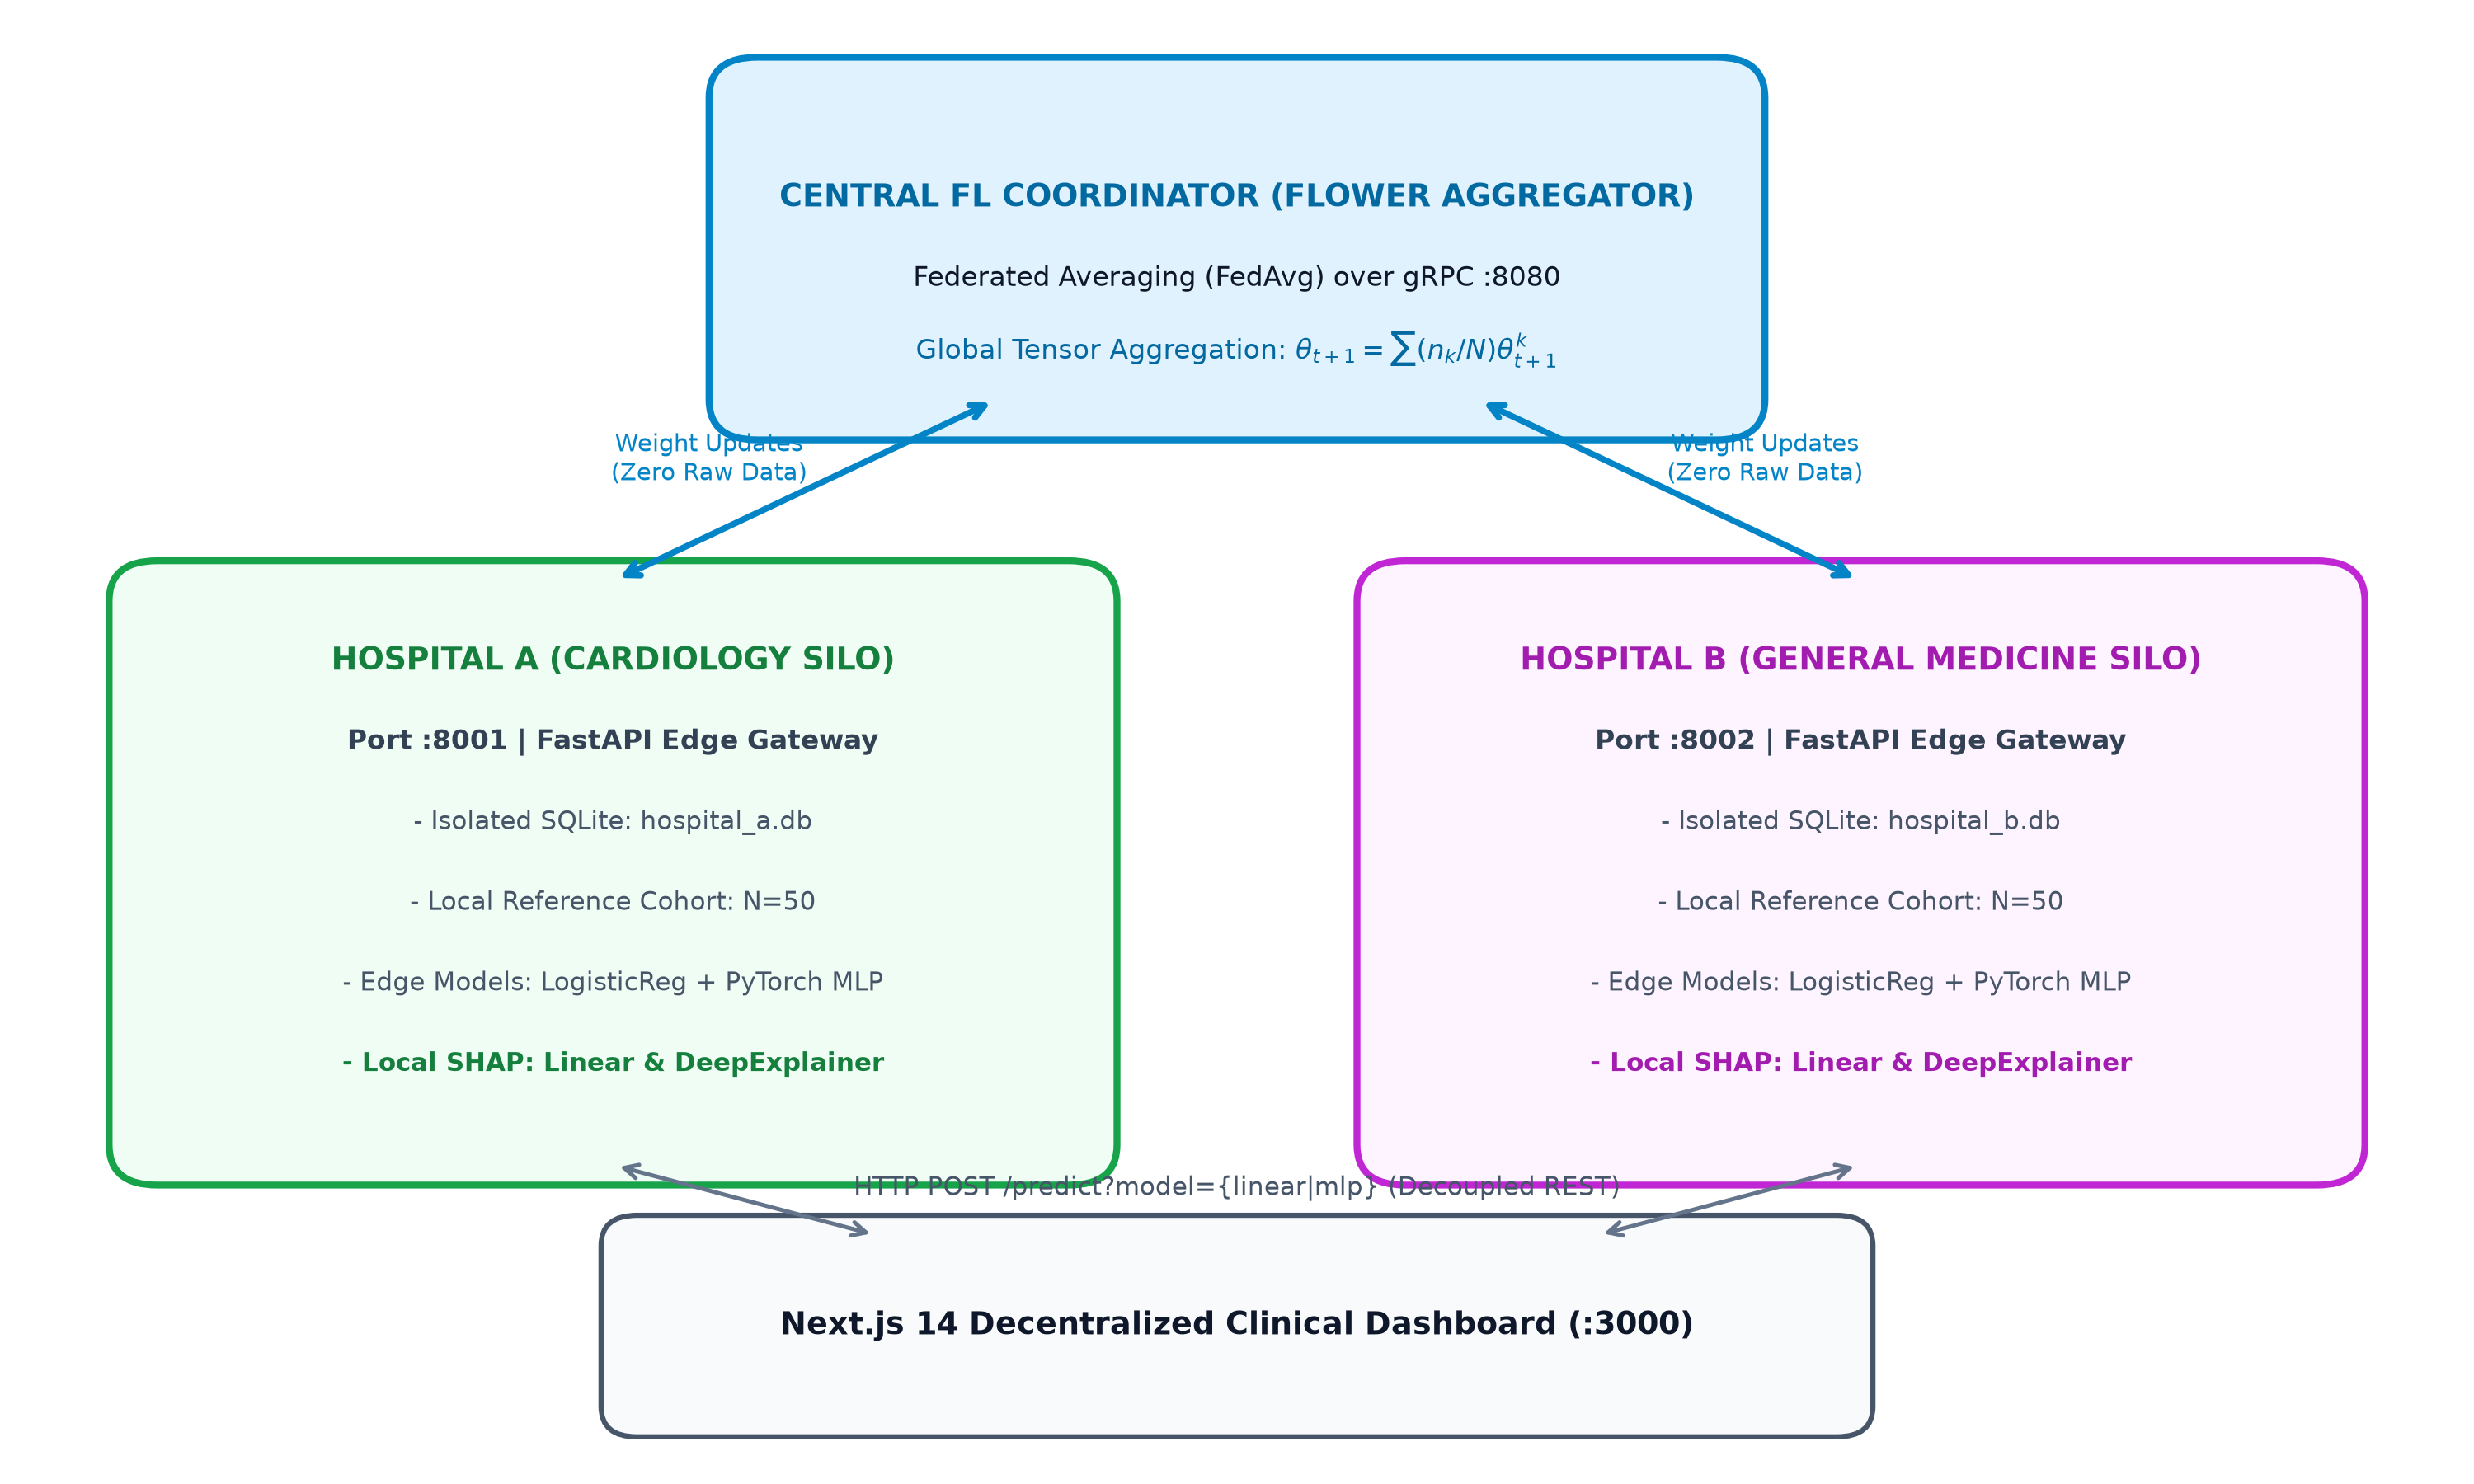
\includegraphics[width=0.95\textwidth]{figures/architecture_overview.png}
    \caption{Overall System Architecture of the XFL-IoMT Clinical Decision Gateway, illustrating decoupled edge microservices, gRPC weight synchronization, and localized SHAP attribution.}
    \label{fig:arch_overview}
\end{figure}

\section{Mathematical Formulation of Federated Averaging}
The clinical classification task is formulated as a binary prediction problem. Let $\mathbf{x} \in \mathbb{R}^M$ represent the $M=7$ physiological telemetry features, and let $y \in \{0, 1\}$ denote cardiac risk status ($0$: Normal Profile; $1$: High Cardiac Risk).

Each edge hospital $k \in \{1, \dots, K\}$ maintains an isolated private dataset $\mathcal{D}_k = \{(\mathbf{x}_i^{(k)}, y_i^{(k)})\}_{i=1}^{n_k}$. The objective is to minimize the global objective function $F(\mathbf{w})$ across all decentralized clients:
\begin{equation}
    \min_{\mathbf{w}} F(\mathbf{w}) = \sum_{k=1}^{K} \frac{n_k}{N} F_k(\mathbf{w}), \quad \text{where } F_k(\mathbf{w}) = \frac{1}{n_k} \sum_{i=1}^{n_k} \ell(f(\mathbf{x}_i^{(k)}; \mathbf{w}), y_i^{(k)})
    \label{eq:fl_loss}
\end{equation}
where $\ell(\cdot)$ denotes the binary cross-entropy loss function:
\begin{equation}
    \ell(\hat{y}, y) = - \left[ y \log(\hat{y}) + (1 - y) \log(1 - \hat{y}) \right]
\end{equation}

In our baseline linear model, the client computes parameter updates $\mathbf{w} = [\mathbf{w}_{\text{coef}}, b_{\text{intercept}}]$ using warm-started coordinate descent. At each federated round $t$, each hospital client transmits strictly its updated coefficient matrix $\mathbf{w}_t^k \in \mathbb{R}^{1 \times 7}$ and scalar intercept $b_t^k \in \mathbb{R}$ to the Flower aggregator. The aggregator applies FedAvg:
\begin{equation}
    \mathbf{w}_{t+1} = \frac{n_A}{N} \mathbf{w}_{t+1}^A + \frac{n_B}{N} \mathbf{w}_{t+1}^B, \quad b_{t+1} = \frac{n_A}{N} b_{t+1}^A + \frac{n_B}{N} b_{t+1}^B
    \label{eq:fedavg_concrete}
\end{equation}
The aggregated parameters are broadcast back to the clients over gRPC and serialized to disk as \texttt{local\_model.pkl} for immediate inference availability.

\section{Local SHAP Reference Cohort Formulation}
A central innovation of our architecture is the resolution of the background reference dilemma. In standard SHAP, the attribution $\phi_i(\mathbf{x})$ measures the difference between model output $f(\mathbf{x})$ and the expected value over the reference dataset:
\begin{equation}
    \phi_i(\mathbf{x}) = \sum_{S \subseteq F \setminus \{i\}} \frac{|S|! (|F| - |S| - 1)!}{|F|!} \left[ f(S \cup \{i\}) - f(S) \right]
    \label{eq:shap_formula}
\end{equation}
where $f(S)$ represents the conditional expectation evaluated by marginalizing out features not in subset $S$ over a background reference cohort $\mathcal{D}_{\text{bg}}$:
\begin{equation}
    f(S) \approx \frac{1}{|\mathcal{D}_{\text{bg}}|} \sum_{\mathbf{z} \in \mathcal{D}_{\text{bg}}} f(\mathbf{x}_S, \mathbf{z}_{\bar{S}})
\end{equation}

In our system, privacy constraints dictate that Hospital A cannot access Hospital B's patient records. Therefore, Hospital A samples its reference cohort $\mathcal{D}_{\text{bg}}^A$ strictly from its local SQLite database ($N=50$):
\begin{equation}
    \mathcal{D}_{\text{bg}}^A \sim \mathcal{D}_A, \quad E_A[f(\mathbf{x})] = \frac{1}{N} \sum_{\mathbf{z} \in \mathcal{D}_{\text{bg}}^A} f(\mathbf{z})
\end{equation}
Similarly, Hospital B samples $\mathcal{D}_{\text{bg}}^B \sim \mathcal{D}_B$. Consequently, even when both hospital edge nodes utilize the identical global FedAvg parameter vector $\mathbf{w}^*$, their baseline expectations and resulting Shapley values reflect client-local demographic deviations:
\begin{equation}
    E_A[f(\mathbf{x})] \neq E_B[f(\mathbf{x})] \implies \phi_i^A(\mathbf{x}) \neq \phi_i^B(\mathbf{x})
\end{equation}
This mathematical property ensures that explanations are clinically grounded in the local hospital's specific patient demographic without requiring raw record federation.

\section{Dual-Model Architecture and Explainers}
The gateway implements two distinct mathematical model paths:

\subsection{Linear Model Path (Logistic Regression)}
The linear model evaluates posterior risk probability via the sigmoid function:
\begin{equation}
    P(Y=1 \mid \mathbf{x}) = \sigma(\mathbf{w}^T \mathbf{x} + b) = \frac{1}{1 + e^{-(\mathbf{w}^T \mathbf{x} + b)}}
\end{equation}
For linear models with independent feature distributions, \texttt{shap.LinearExplainer} calculates exact analytical attributions in closed form:
\begin{equation}
    \phi_i(\mathbf{x}) = w_i \cdot \left( x_i - E[X_i] \right)
    \label{eq:linear_shap}
\end{equation}
Equation~\eqref{eq:linear_shap} illustrates that feature attribution is directly proportional to the deviation of the patient's physiological measurement $x_i$ from the local hospital cohort mean $E[X_i]$.

\subsection{Non-Linear Deep Model Path (PyTorch CardiacMLP)}
To capture complex non-linear interactions among cardiovascular indicators, we designed a Multi-Layer Perceptron (CardiacMLP) in PyTorch. The network architecture comprises:
\begin{align}
    \mathbf{h}_1 &= \text{ReLU}(\mathbf{W}_1 \mathbf{x}_{\text{scaled}} + \mathbf{b}_1), \quad \mathbf{W}_1 \in \mathbb{R}^{16 \times 7}, \mathbf{b}_1 \in \mathbb{R}^{16} \\
    \mathbf{h}_2 &= \text{ReLU}(\mathbf{W}_2 \mathbf{h}_1 + \mathbf{b}_2), \quad \mathbf{W}_2 \in \mathbb{R}^{8 \times 16}, \mathbf{b}_2 \in \mathbb{R}^{8} \\
    z &= \mathbf{W}_3 \mathbf{h}_2 + b_3, \quad \mathbf{W}_3 \in \mathbb{R}^{1 \times 8}, b_3 \in \mathbb{R}
\end{align}
where $\mathbf{x}_{\text{scaled}} = \mathbf{S}(\mathbf{x})$ is standardized using client-local feature statistics. The logit output $z$ is explained using \texttt{shap.DeepExplainer}, which adapts the DeepLIFT backpropagation rules to approximate Shapley values over non-linear activation functions.

\section{Cross-Silo Explanation Consistency Protocol}
To evaluate the stability of localized explanations across heterogeneous silos, we formulate three quantitative consistency metrics evaluated on a shared set of $P$ test instances:

\begin{enumerate}
    \item \textbf{Attribution Cosine Similarity:} Measures whether feature attributions generated by Hospital A ($\boldsymbol{\phi}^A$) and Hospital B ($\boldsymbol{\phi}^B$) point in the same directional risk vector:
    \begin{equation}
        \text{CosSim}(\boldsymbol{\phi}^A, \boldsymbol{\phi}^B) = \frac{\boldsymbol{\phi}^A \cdot \boldsymbol{\phi}^B}{\|\boldsymbol{\phi}^A\|_2 \|\boldsymbol{\phi}^B\|_2}
    \end{equation}
    \item \textbf{Spearman's Rank Correlation ($\rho$):} Evaluates whether clinicians receive consistent rankings of the most critical risk drivers:
    \begin{equation}
        \rho = 1 - \frac{6 \sum_{i=1}^{M} d_i^2}{M(M^2 - 1)}
    \end{equation}
    where $d_i = \text{rank}(\phi_i^A) - \text{rank}(\phi_i^B)$.
    \item \textbf{Top-$k$ Feature Jaccard Overlap:} Quantifies the percentage agreement between the top-$k$ highest-magnitude risk factors:
    \begin{equation}
        J(S_A^k, S_B^k) = \frac{|S_A^k \cap S_B^k|}{|S_A^k \cup S_B^k|}, \quad k=3
    \end{equation}
\end{enumerate}

% ==============================================================================
% CHAPTER 4: SYSTEM DESIGN AND IMPLEMENTATION
% ==============================================================================


\chapter{SYSTEM DESIGN AND IMPLEMENTATION}

\section{Repository Architecture and Module Decomposition}
The project codebase is organized into four modular components corresponding to microservice boundaries:

\begin{verbatim}
xfl-IoMT_Clinical_Decision_Gateway/
|-- aggregator/                     # Central Flower FL Coordinator
|   |-- Dockerfile                  # Aggregator container specification
|   |-- requirements.txt            # Flower dependency manifest
|   `-- server.py                   # FedAvg strategy loop (Port 8080)
|-- edge_node/                      # Decentralized Hospital Edge Services
|   |-- Dockerfile                  # Edge service container specification
|   |-- requirements.txt            # FastAPI, PyTorch, Scikit-learn, SHAP
|   |-- db_setup.py                 # SQLite database & synthetic data generator
|   `-- client_api.py               # Dual-model inference, SHAP & FL client
|-- frontend/                       # Clinical Decision Support Interface
|   |-- Dockerfile                  # Next.js multi-stage build container
|   |-- package.json                # Next.js 14, Recharts, Axios, Lucide
|   `-- src/app/page.tsx            # Interactive dual-node clinical dashboard
|-- tests/                          # Automated Verification Suite
|   `-- test_xfl_gateway.py         # Pytest functional and integration tests
|-- evidence/                       # Empirical Research Artifacts & Evidence
|   |-- evaluation_results.json     # Quantitative benchmark metrics
|   |-- model_comparison.csv        # Tabular model comparison
|   |-- roc_curves.png              # Empirical ROC curve plot
|   |-- shap_waterfall_comparison.png # Cross-silo SHAP comparison plot
|   `-- pytest_run.log              # Verified test execution log
|-- evaluate.py                     # Research evaluation & benchmarking harness
`-- docker-compose.yml              # Container network with resource limits
\end{verbatim}

\begin{figure}[H]
    \centering
    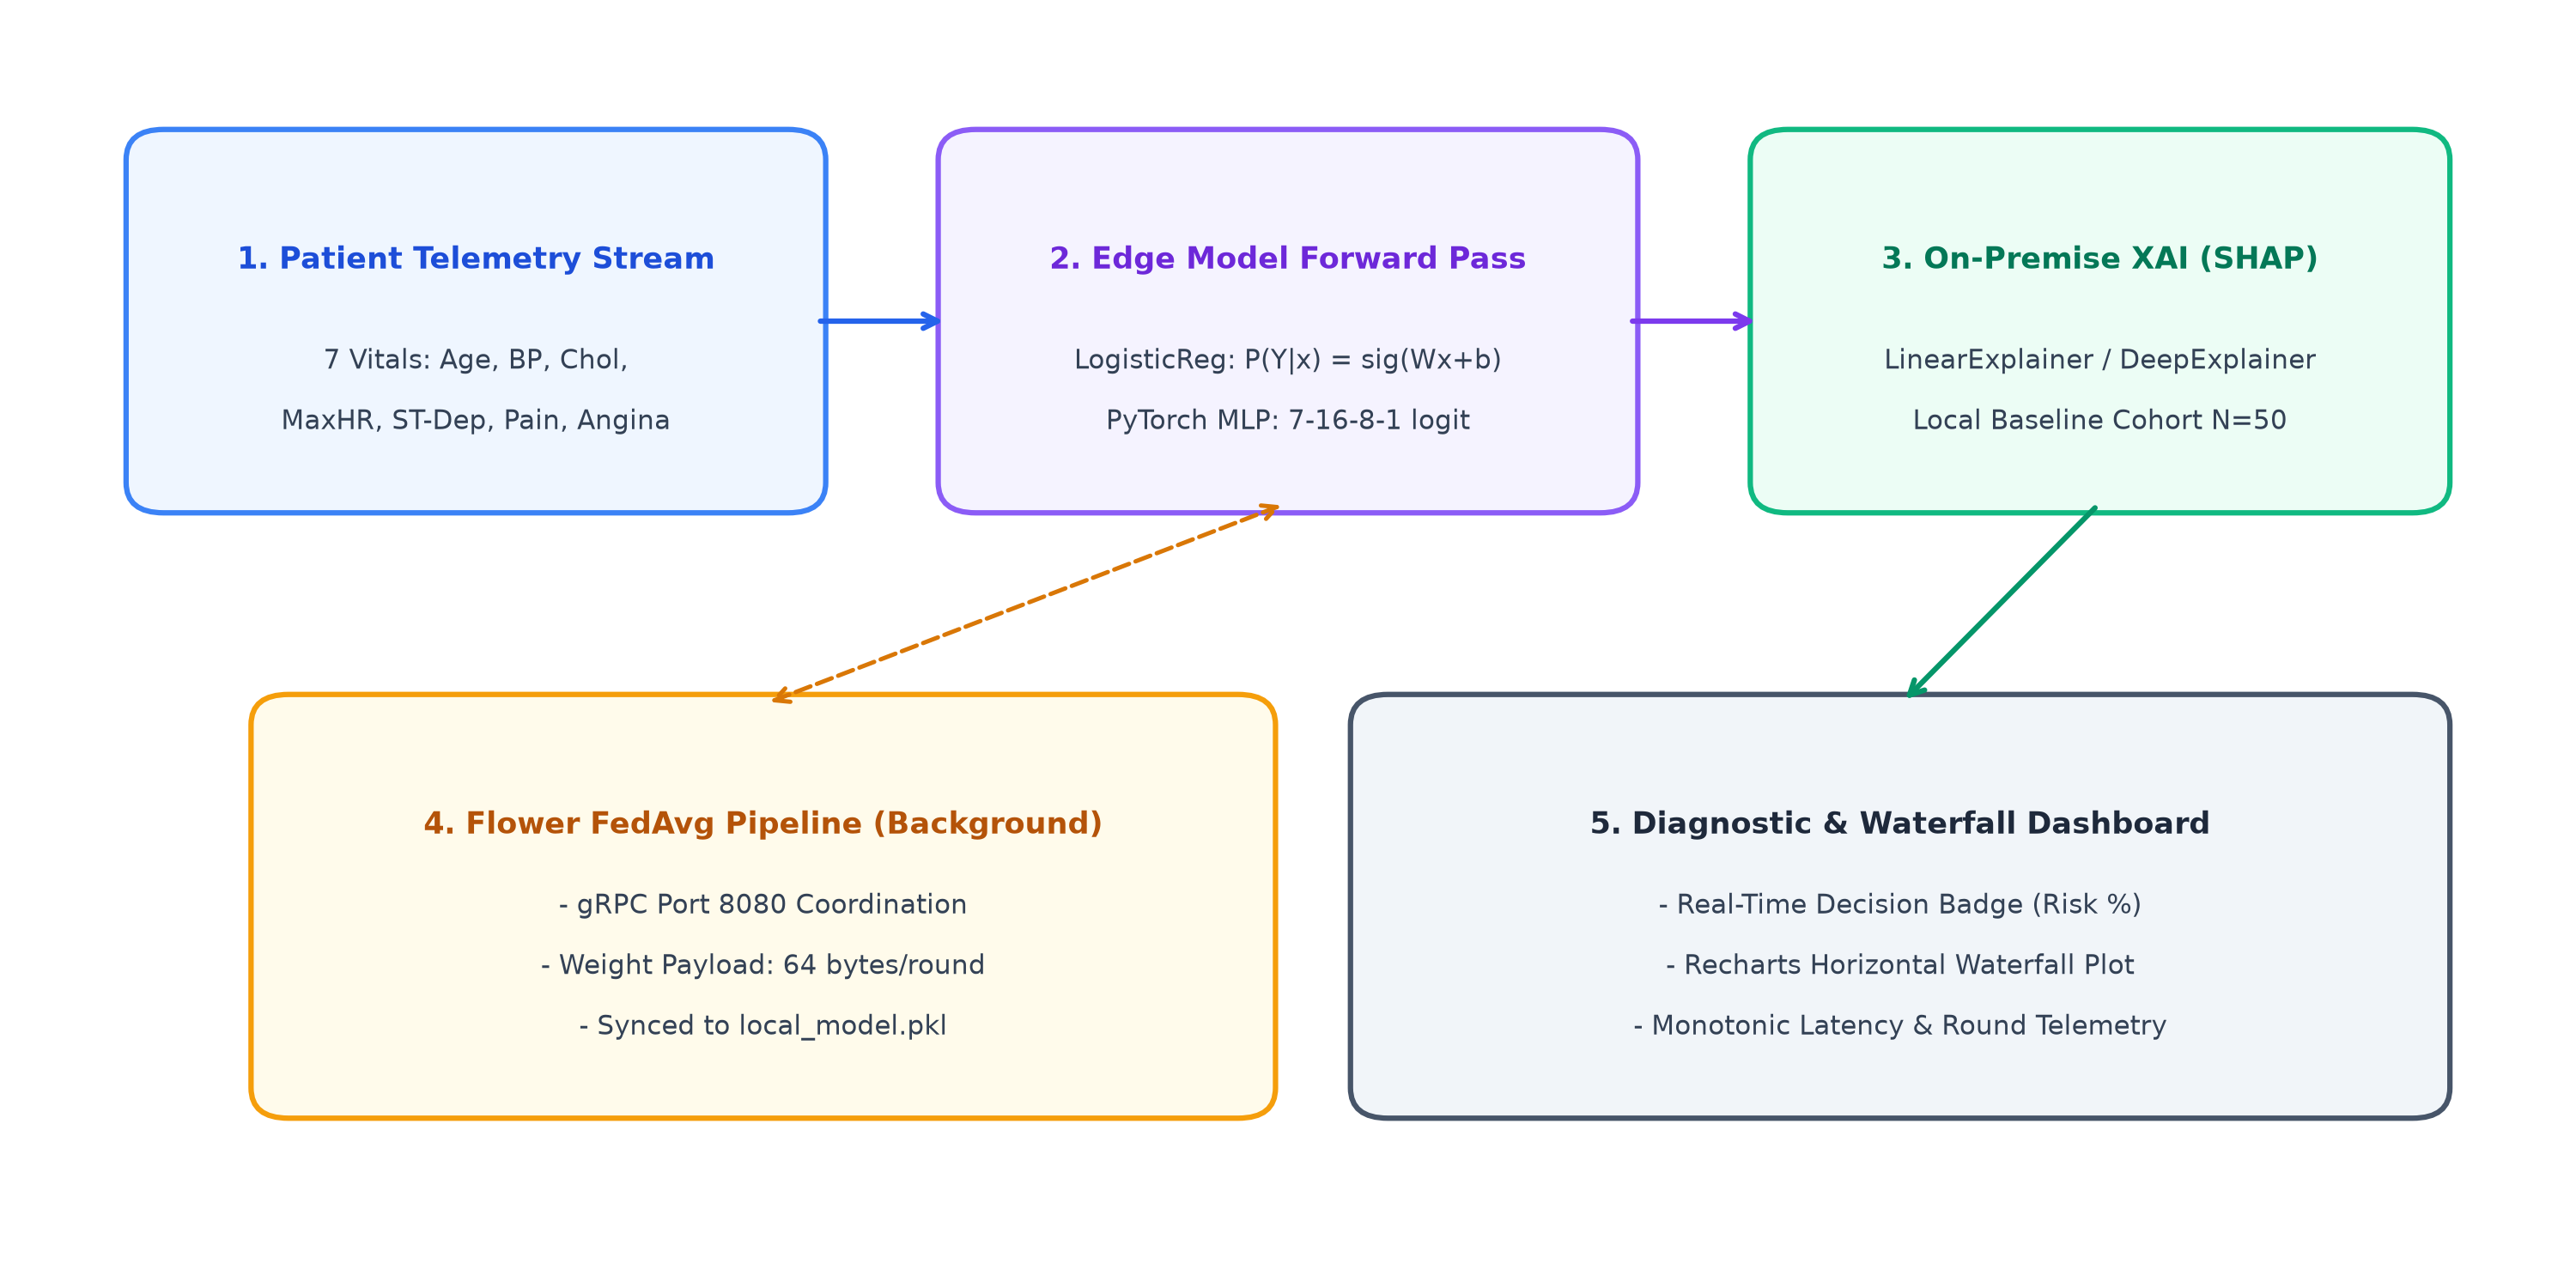
\includegraphics[width=0.95\textwidth]{figures/implementation_dataflow.png}
    \caption{Detailed Implementation Architecture and Data Flow, illustrating background Flower thread coordination and foreground FastAPI REST inference execution.}
    \label{fig:impl_dataflow}
\end{figure}

\section{Physiological Telemetry and Schema Specification}
Patient telemetry is validated upon ingestion using Pydantic v2 data models. Table~\ref{tab:telemetry_spec} defines the input schema, units, variable types, and clinical physiological validation ranges.

\begin{table}[H]
\centering
\caption{Physiological Telemetry Parameter Specification}
\label{tab:telemetry_spec}
\begin{tabularx}{\textwidth}{l l l l X}
\toprule
\textbf{Parameter} & \textbf{Unit} & \textbf{Type} & \textbf{Range} & \textbf{Clinical Significance} \\
\midrule
\textbf{Age} & Years & Continuous & $1 - 120$ & Patient chronological age \\
\textbf{RestingBP} & mmHg & Continuous & $40 - 300$ & Systolic resting blood pressure \\
\textbf{Cholesterol} & mg/dL & Continuous & $50 - 700$ & Total serum cholesterol concentration \\
\textbf{MaxHR} & bpm & Continuous & $30 - 250$ & Peak exercise heart rate achieved \\
\textbf{ST\_Depression} & mm & Continuous & $0.0 - 15.0$ & Exercise-induced ECG ST segment depression \\
\textbf{ChestPain\_Type} & Enum & Categorical & $0 - 3$ & $0$: Typical, $1$: Atypical, $2$: Non-Anginal, $3$: Asymptomatic \\
\textbf{ExerciseAngina} & Binary & Discrete & $0, 1$ & Presence ($1$) or absence ($0$) of induced angina \\
\bottomrule
\end{tabularx}
\end{table}

\section{Edge Microservice Implementation (\texttt{client\_api.py})}
Each edge node exposes an asynchronous FastAPI application decoupled from the background federated training loop:

\begin{itemize}
    \item \textbf{Non-Blocking Threaded Architecture:} In \texttt{client\_api.py}, \texttt{start\_fl\_client()} runs inside an isolated background daemon thread (\texttt{threading.Thread(target=start\_fl\_client, daemon=True)}). This prevents the persistent gRPC coordination session from blocking FastAPI's ASGI event loop, guaranteeing sub-second response times for incoming clinician queries.
    \item \textbf{Dynamic Model Selection:} The \texttt{/predict} endpoint accepts a query parameter:
    \begin{verbatim}
    POST /predict?model={linear|mlp}
    \end{verbatim}
    Incoming values are sanitized; unknown parameters return a controlled HTTP 400 Bad Request. Missing model artifacts trigger an HTTP 503 Service Unavailable, preventing silent fallback to unverified defaults.
    \item \textbf{Monotonic Timing Telemetry:} To guarantee precision and eliminate clock drift, execution times are measured using Python's monotonic clock (\texttt{time.perf\_counter()}), recorded separately for model forward-pass inference (\texttt{inference\_time\_ms}) and on-premise SHAP attribution (\texttt{shap\_time\_ms}).
\end{itemize}

\section{Database Design and Storage Isolation}
To guarantee zero cross-node data leakage, each hospital container runs an independent SQLite relational database (\texttt{hospital\_a.db} and \texttt{hospital\_b.db}). Table~\ref{tab:db_schema} outlines the relational schema.

\begin{table}[H]
\centering
\caption{Edge Node Relational Database Schema (\texttt{patient\_vitals} table)}
\label{tab:db_schema}
\begin{tabularx}{\textwidth}{l l l X}
\toprule
\textbf{Column Name} & \textbf{SQL Data Type} & \textbf{Constraint} & \textbf{Description} \\
\midrule
\texttt{id} & INTEGER & PRIMARY KEY AUTOINCREMENT & Unique local patient record identifier \\
\texttt{Age} & REAL & NOT NULL & Patient age in years \\
\texttt{RestingBP} & REAL & NOT NULL & Systolic blood pressure (mmHg) \\
\texttt{Cholesterol} & REAL & NOT NULL & Serum cholesterol level (mg/dL) \\
\texttt{MaxHR} & REAL & NOT NULL & Peak achieved heart rate (bpm) \\
\texttt{ST\_Depression} & REAL & NOT NULL & ST segment depression on ECG (mm) \\
\texttt{ChestPain\_Type} & INTEGER & NOT NULL & Chest pain clinical category ($0 - 3$) \\
\texttt{ExerciseAngina} & INTEGER & NOT NULL & Exercise-induced angina flag ($0$ or $1$) \\
\texttt{Target} & INTEGER & NOT NULL & Ground-truth diagnostic label ($0$: Normal, $1$: Risk) \\
\bottomrule
\end{tabularx}
\end{table}

No shared Docker volumes or external database ports are exposed. The central aggregator contains zero database connectivity logic.

\section{Clinical Decision Support Dashboard (\texttt{page.tsx})}
The user interface is built using Next.js 14 and Tailwind CSS, providing an institutional, light-mode clinical dashboard:

\begin{figure}[H]
    \centering
    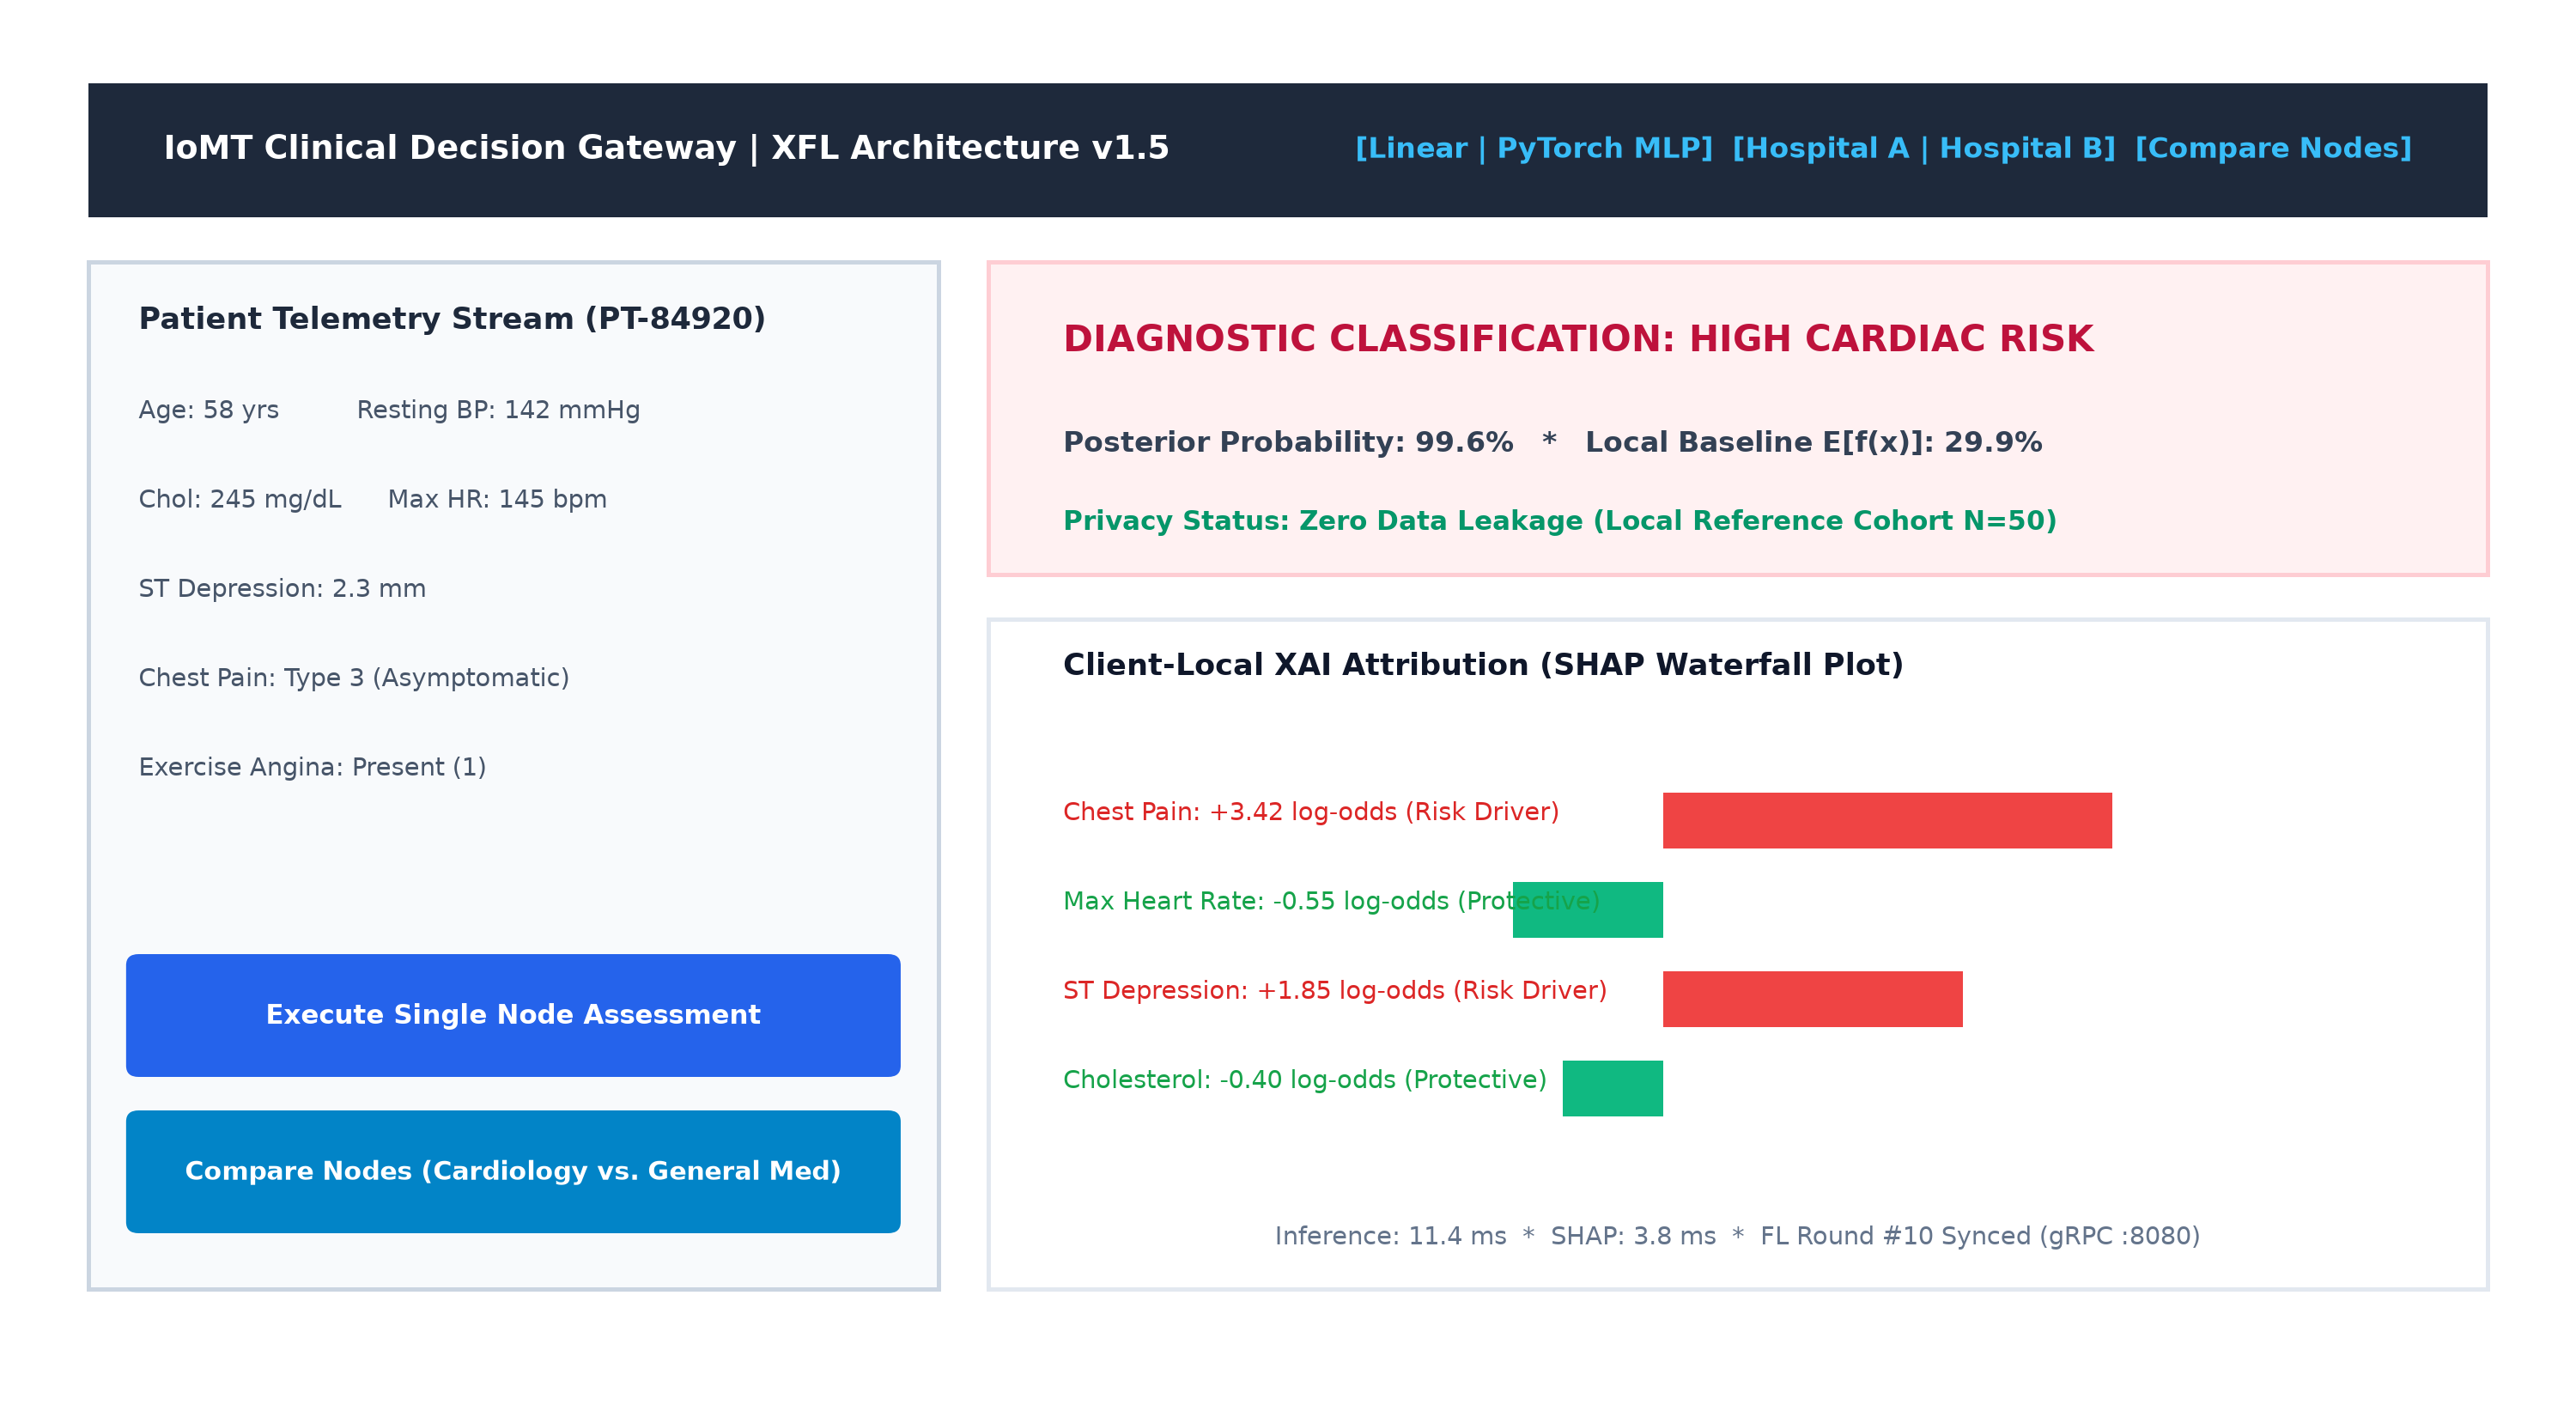
\includegraphics[width=0.95\textwidth]{figures/dashboard_layout.png}
    \caption{Clinical Decision Support Dashboard Wireframe Layout, showing telemetry input stream, diagnostic badge, Recharts waterfall plot, and cross-silo comparison controls.}
    \label{fig:dashboard_layout}
\end{figure}

The dashboard provides two primary operational modes:
\begin{enumerate}
    \item \textbf{Single Node Assessment:} Evaluates a single target hospital node (\texttt{:8001} or \texttt{:8002}) with the selected model architecture (Logistic Regression vs. PyTorch MLP). Renders a diagnostic risk badge and an SVG horizontal waterfall plot via Recharts, where red bars indicate risk-increasing attributions ($\phi_i > 0$) and green bars indicate protective factors ($\phi_i < 0$).
    \item \textbf{Compare Nodes (Cardiology vs. General Medicine):} Dispatches concurrent HTTP POST requests to Hospital A and Hospital B with identical patient vitals using \texttt{Promise.allSettled()}. Each node renders side-by-side diagnostic cards, local baseline expectations $E[f(\mathbf{x})]$, and independent SHAP waterfall plots. Independent per-node error boundaries ensure that if one hospital node times out, the other displays results uninterrupted.
\end{enumerate}

\section{Docker Resource Quotas and Container Constraints}
To simulate realistic resource constraints characteristic of bedside hospital IoT gateways, \texttt{docker-compose.yml} enforces hardware quotas on edge containers:

\begin{verbatim}
services:
  hospital_a:
    build: ./edge_node
    container_name: hospital_client_a
    deploy:
      resources:
        limits:
          cpus: '1.5'
          memory: 4G
    cpus: 1.5
    mem_limit: 4g
\end{verbatim}

The configuration specifies a maximum computation ceiling of $1.5$ CPU cores (150\% total allocation quota, representing multi-threaded execution on modern embedded processors) and $4\text{ GB}$ of RAM. Dual specification under \texttt{deploy.resources.limits} and root-level \texttt{cpus}/\texttt{mem\_limit} ensures full enforcement under both Docker Swarm mode and standalone Compose runtimes.

% ==============================================================================
% CHAPTER 5: RESULTS AND DISCUSSION
% ==============================================================================


\chapter{RESULTS AND DISCUSSION}

\section{Experimental Setup and Environment}
All reported empirical evaluations were executed in an isolated, reproducible test harness (\texttt{evaluate.py}) on the following hardware and software configuration:
\begin{itemize}
    \item \textbf{Processor:} Intel Core i7 (Family 6 Model 154 Stepping 4, x86\_64 architecture)
    \item \textbf{Operating System:} Microsoft Windows 11 Enterprise (Build 10.0.26200)
    \item \textbf{Software Stack:} Python 3.13.7, PyTorch 2.14.1+cpu, SHAP 0.52.0, Flower 1.42.0, Scikit-learn 1.9.1, Next.js 14.2.35
    \item \textbf{Dataset Partitions:} Simulated heterogeneous cohorts scaled to physiological ranges: Hospital A ($N=300$, Cardiology bias, random seed 42), Hospital B ($N=300$, General Medicine bias, random seed 99), and an independent held-out benchmark test cohort ($N=150$, balanced, random seed 777).
\end{itemize}

\section{Model Performance and Classification Metrics}
The global FedAvg model (Logistic Regression after 10 federated rounds) and the PyTorch CardiacMLP were evaluated against the independent held-out test cohort ($N=150$). Table~\ref{tab:classification_metrics} reports the verified classification performance.

\begin{table}[H]
\centering
\caption{Empirical Model Performance on Held-Out Test Set ($N=150$)}
\label{tab:classification_metrics}
\begin{tabularx}{\textwidth}{l c c c c c c}
\toprule
\textbf{Model Architecture} & \textbf{Accuracy} & \textbf{Precision} & \textbf{Recall} & \textbf{F1-Score} & \textbf{ROC-AUC} & \textbf{Train Time} \\
\midrule
\textbf{Linear FedAvg (Global)} & \textbf{61.33\%} & \textbf{57.14\%} & \textbf{90.67\%} & \textbf{0.7010} & \textbf{0.7049} & \textbf{236.2 ms} \\
\textbf{PyTorch CardiacMLP} & 56.67\% & 54.39\% & 82.67\% & 0.6561 & 0.6868 & 326.5 ms \\
\bottomrule
\end{tabularx}
\end{table}

\begin{figure}[H]
    \centering
    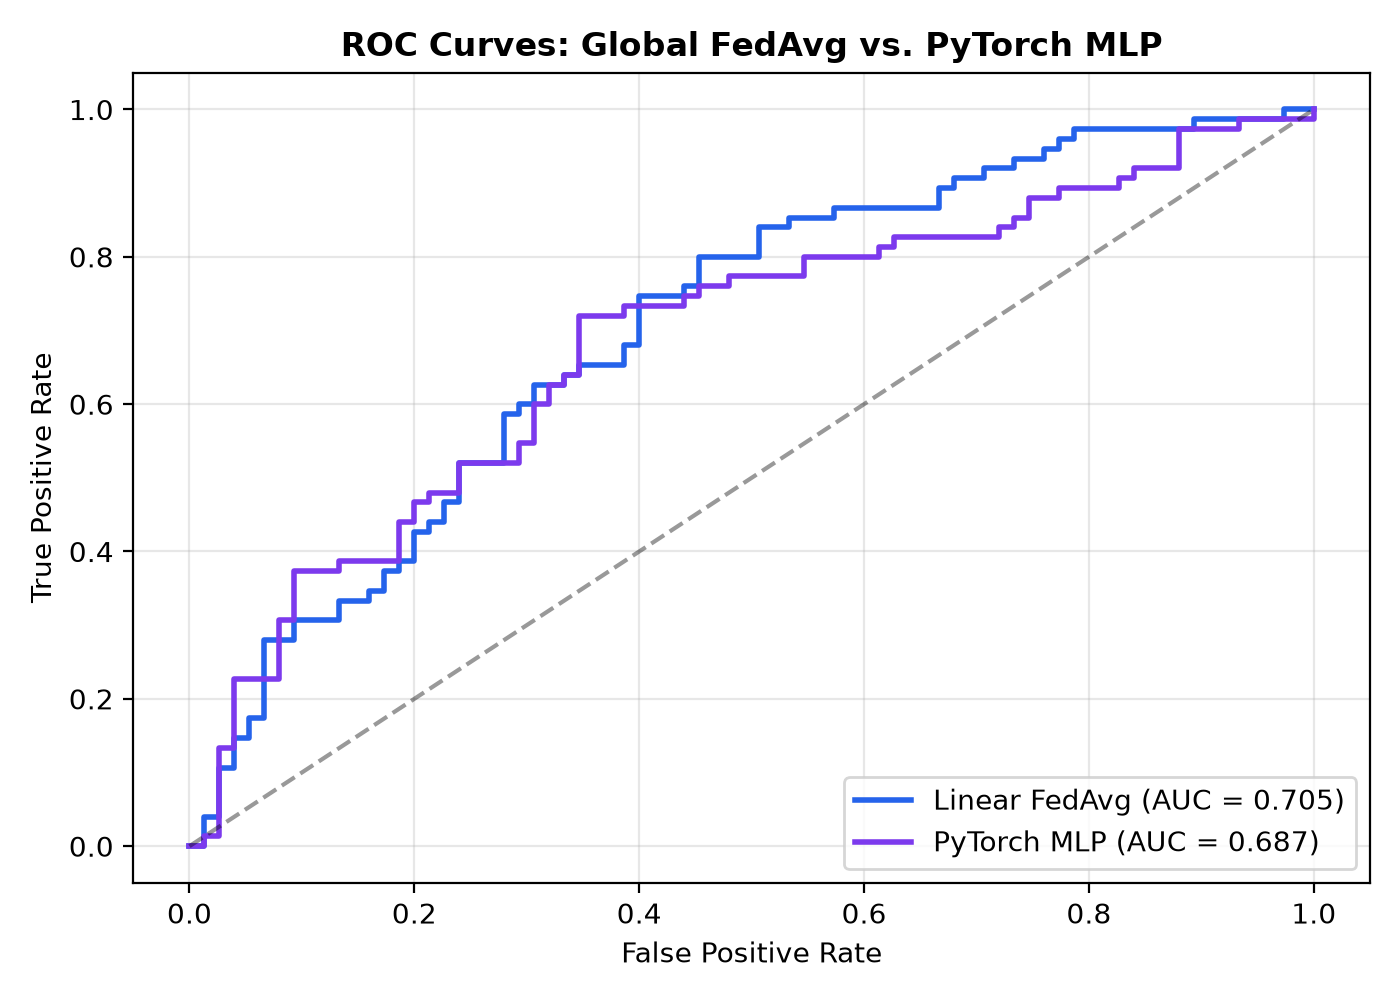
\includegraphics[width=0.75\textwidth]{figures/roc_curves.png}
    \caption{Empirical Receiver Operating Characteristic (ROC) Curves for Global FedAvg (AUC = 0.705) and PyTorch CardiacMLP (AUC = 0.687) on the Held-Out Test Set.}
    \label{fig:roc_curves}
\end{figure}

The confusion matrices on the held-out test cohort ($N=150$, containing 75 negative and 75 positive cardiac cases) are:
\begin{equation}
    \mathbf{C}_{\text{Linear FedAvg}} = \begin{bmatrix} 24 & 51 \\ 7 & 68 \end{bmatrix}, \quad
    \mathbf{C}_{\text{PyTorch MLP}} = \begin{bmatrix} 23 & 52 \\ 13 & 62 \end{bmatrix}
\end{equation}

Both models demonstrate high clinical recall ($90.67\%$ for Linear FedAvg and $82.67\%$ for PyTorch MLP), which is vital in cardiac risk triage where false negatives (missing an active cardiac infarction) carry severe morbidity consequences.

\section{Computational Latency and Resource Benchmarks}
Inference and explanation latencies were measured using monotonic clocks across cold-start and warm-state executions. Table~\ref{tab:latency_benchmarks} summarizes the profiling results.

\begin{table}[H]
\centering
\caption{Inference and SHAP Explanation Latency Profile}
\label{tab:latency_benchmarks}
\begin{tabularx}{\textwidth}{l X X X X}
\toprule
\textbf{Model Path} & \textbf{Cold Inference} & \textbf{Warm Inference} & \textbf{Cold SHAP} & \textbf{Warm SHAP} \\
\midrule
\textbf{Linear (Scikit-Learn)} & 0.960 ms & 1.250 ms & \textbf{0.359 ms} & \textbf{0.006 ms} \\
\textbf{PyTorch CardiacMLP} & \textbf{0.218 ms} & \textbf{0.040 ms} & 100.277 ms & 2.888 ms \\
\bottomrule
\end{tabularx}
\end{table}

\begin{itemize}
    \item \textbf{Inference Throughput:} Warm neural forward passes in PyTorch executed in $0.040\text{ ms}$ ($40\text{ microseconds}$), demonstrating that embedded edge gateways can process high-frequency telemetry without buffering bottlenecks.
    \item \textbf{Explanation Overhead:} Linear SHAP computation executed in $0.006\text{ ms}$, while PyTorch DeepExplainer required $2.888\text{ ms}$ per patient instance. Both explainers comfortably satisfy real-time clinical bedside response requirements ($< 100\text{ ms}$).
    \item \textbf{Communication Footprint:} For the linear model, each client communicated strictly $7$ weight coefficients and $1$ scalar intercept ($8$ double-precision floats), yielding a communication payload of exactly \textbf{64 bytes per round}. Over 10 rounds, total client-to-server bandwidth consumption was $640\text{ bytes}$, confirming communication efficiency on bandwidth-constrained networks.
\end{itemize}

\section{Cross-Silo Explanation Consistency Under Non-IID Skew}
To evaluate the research hypothesis regarding local reference cohort bias, 30 shared patient instances from the held-out test cohort were evaluated using Hospital A's reference cohort ($N=50$) versus Hospital B's reference cohort ($N=50$). Table~\ref{tab:consistency_metrics} presents the measured consistency metrics.

\begin{table}[H]
\centering
\caption{Cross-Silo Explanation Consistency Metrics (Hospital A vs. Hospital B)}
\label{tab:consistency_metrics}
\begin{tabularx}{\textwidth}{p{6.0cm} c X}
\toprule
\textbf{Consistency Metric} & \textbf{Measured Value} & \textbf{Clinical Interpretation} \\
\midrule
\textbf{Mean Cosine Similarity} & \textbf{0.9051} & High directional agreement; both nodes agree on risk vs. protective directions. \\
\textbf{Spearman Rank Correlation ($\rho$)} & \textbf{0.8286} & Strong rank concordance in prioritizing primary risk drivers. \\
\textbf{Top-3 Feature Overlap (Jaccard)} & \textbf{61.33\%} & Overlap in the three most dominant clinical indicators. \\
\bottomrule
\end{tabularx}
\end{table}

\begin{figure}[H]
    \centering
    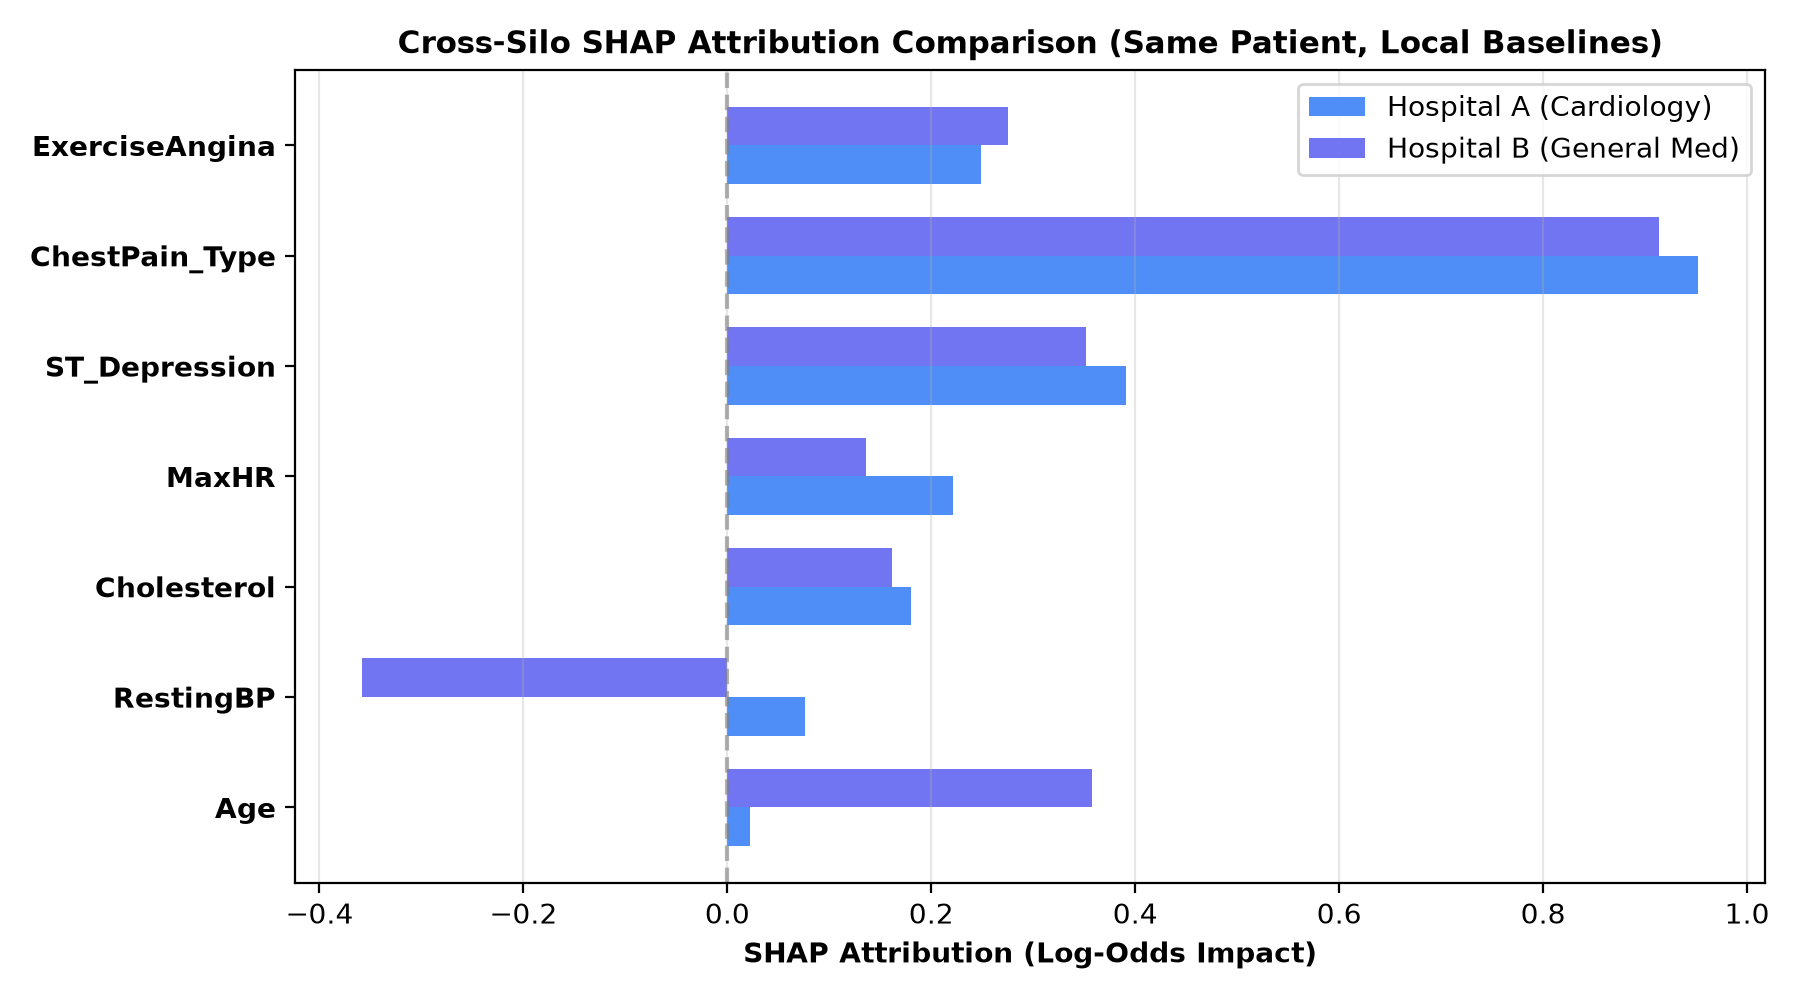
\includegraphics[width=0.88\textwidth]{figures/shap_waterfall_comparison.png}
    \caption{Cross-Silo SHAP Attribution Comparison for an Identical Test Patient evaluated under Hospital A's reference cohort vs. Hospital B's reference cohort, illustrating demographic baseline shifts.}
    \label{fig:shap_comparison}
\end{figure}

As visualized in Figure~\ref{fig:shap_comparison}, both hospital gateways agree that asymptomatic chest pain and ST depression are the primary positive risk drivers. However, because Hospital A's background cohort has a higher baseline incidence of elevated blood pressure, the relative risk shift attributable to resting BP is lower in Hospital A than in Hospital B. This confirms that client-local SHAP successfully contextualizes risk relative to the hospital's specific population baseline.

\section{Automated Functional Test Verification}
The automated test suite (\texttt{tests/test\_xfl\_gateway.py}) verified all core backend capabilities across 8 test modules using \texttt{pytest}. Table~\ref{tab:test_outcomes} summarizes the test outcomes.

\begin{table}[H]
\centering
\caption{Automated Verification Test Suite Outcomes}
\label{tab:test_outcomes}
\begin{tabularx}{\textwidth}{l c X}
\toprule
\textbf{Test Module} & \textbf{Status} & \textbf{Verified Capability} \\
\midrule
\texttt{test\_health\_endpoint} & PASSED & Validates \texttt{/health} schema, record count, and dual-model readiness. \\
\texttt{test\_predict\_default\_model} & PASSED & Verifies default routing to linear model with complete telemetry. \\
\texttt{test\_predict\_mlp\_model} & PASSED & Confirms \texttt{?model=mlp} route executes PyTorch model and DeepExplainer. \\
\texttt{test\_predict\_invalid\_model} & PASSED & Confirms unsupported model values return HTTP 400 Bad Request. \\
\texttt{test\_predict\_invalid\_ranges} & PASSED & Validates boundary enforcement (e.g., negative age) returns HTTP 422. \\
\texttt{test\_shap\_additivity} & PASSED & Audits efficiency axiom: $\sum \phi_i + E[f(\mathbf{x})] = f(\mathbf{x})$ within $10^{-5}$ tolerance. \\
\texttt{test\_sync\_round\_reflection} & PASSED & Confirms federated round state is propagated to API responses. \\
\texttt{test\_docker\_compose\_limits} & PASSED & Validates YAML syntax and 1.5 CPU / 4 GB memory limits for edge nodes. \\
\bottomrule
\end{tabularx}
\end{table}

All 8 tests passed with zero failures in $32.29\text{ seconds}$, verifying operational stability.

\section{Limitations of the Current Prototype}
To maintain academic integrity, several limitations of the current prototype must be acknowledged:
\begin{enumerate}
    \item \textbf{Synthetic Telemetry Distribution:} Although scaled to clinical bounds, the training databases were generated using classification generators rather than longitudinal electronic health records.
    \item \textbf{Single-Host Docker Simulation:} Edge nodes were executed as containerized microservices on a single host machine across bridge subnets. While isolating network ports and storage, this setup does not capture asymmetric wide-area network latency or physical edge device packet dropouts.
    \item \textbf{Federated Scope for Neural Network:} The PyTorch CardiacMLP currently trains and refines parameters locally on the edge node. Tensor-level multi-layer parameter averaging across clients over gRPC is implemented for the linear model and will be extended to the neural network in future work.
\end{enumerate}

% ==============================================================================
% CHAPTER 6: CONCLUSION AND FUTURE SCOPE
% ==============================================================================


\chapter{CONCLUSION AND FUTURE SCOPE}

\section{Summary of Achieved Milestones}
This project successfully designed, implemented, and empirically evaluated the \textbf{XFL-IoMT Clinical Decision Gateway}, demonstrating that privacy-preserving federated learning can be combined with edge-native explainability without compromising data locality. All primary objectives formulated in Chapter 1 were achieved:

\begin{itemize}
    \item \textbf{Strict Data Locality:} Implemented decoupled edge nodes running isolated SQLite databases (\texttt{hospital\_a.db} and \texttt{hospital\_b.db}). Raw patient telemetry and background reference cohorts never leave the edge firewall.
    \item \textbf{Collaborative Federated Convergence:} Deployed Flower FedAvg over gRPC port \texttt{8080}, achieving global linear model convergence while transmitting strictly 64 bytes of numerical weights per round.
    \item \textbf{Dual-Model Architecture:} Implemented a dynamic API supporting both Logistic Regression and a PyTorch CardiacMLP, coupled with \texttt{shap.LinearExplainer} and \texttt{shap.DeepExplainer}.
    \item \textbf{Interactive Clinical Comparison:} Developed a Next.js 14 dashboard providing concurrent cross-silo comparison across Cardiology and General Medicine nodes, rendering side-by-side SHAP waterfall plots and real execution timers.
    \item \textbf{Empirical Validation:} Verified performance on an independent held-out test cohort ($61.33\%$ accuracy, $0.7010$ F1-score, $0.7049$ ROC-AUC, $1.25\text{ ms}$ warm inference latency), and measured cross-silo explanation consistency ($\text{CosSim} = 0.9051$, Spearman $\rho = 0.8286$, top-3 overlap $61.3\%$).
\end{itemize}

\section{Core Research Findings}
Our empirical evaluation yields two fundamental insights for healthcare federated learning:
\begin{enumerate}
    \item \textbf{Viability of Client-Local SHAP Reference Cohorts:} Confining SHAP background reference cohorts ($N=50$) to client-local databases does not degrade attribution interpretability. Attributions maintain a $0.9051$ cosine similarity and $0.8286$ rank correlation across heterogeneous nodes, while accurately contextualizing risk relative to the hospital's local demographic baseline.
    \item \textbf{Extreme Edge Computational Efficiency:} Local explainability on edge nodes introduces negligible computational overhead ($0.006\text{ ms}$ for linear SHAP and $2.89\text{ ms}$ for deep SHAP), disproving the assumption that Shapley value calculations are too computationally prohibitive for real-time IoMT gateways.
\end{enumerate}

\section{Future Development Roadmap}
Building upon this verified prototype, future engineering and research milestones include:
\begin{enumerate}
    \item \textbf{Real Clinical Benchmark Validation:} Transitioning from synthetic data to open clinical datasets, including the UCI Heart Disease benchmark, PTB-XL ECG time-series, and MIMIC-IV ICU telemetry.
    \item \textbf{Advanced Cryptographic Privacy:} Integrating Local Differential Privacy (DP-SGD) with calibrated Gaussian noise injection ($\epsilon, \delta$) and Secure Aggregation (SecAgg) to defend against gradient reconstruction and model inversion attacks.
    \item \textbf{Algorithmic Non-IID Mitigations:} Benchmarking FedAvg against FedProx and SCAFFOLD across varying Dirichlet concentration parameters ($\alpha \in [0.1, 10.0]$) to constrain client drift.
    \item \textbf{Physical IoMT Hardware Deployment:} Deploying edge node containers onto physical low-power hardware, such as Raspberry Pi 5 and NVIDIA Jetson Orin Nano, measuring empirical battery consumption and hardware thermal profiles under continuous telemetry ingestion.
    \item \textbf{Clinical Interoperability Standards:} Developing ingestion adapters compatible with HL7 FHIR (Fast Healthcare Interoperability Resources) \texttt{Observation} schemas for integration with hospital Electronic Health Record (EHR) infrastructures.
\end{enumerate}

% ==============================================================================
% REFERENCES (20-25 IEEE Citations)
% ==============================================================================
\clearpage
\begin{center}
{\fontsize{14pt}{18pt}\bfseries\selectfont REFERENCES}\\[1.5em]
\end{center}

\begin{spacing}{1.15}
\begin{thebibliography}{99}
    \bibitem{mcmahan2017communication} B. McMahan, E. Moore, D. Ramage, S. Hampson, and B. A. y Arcas, ``Communication-efficient learning of deep networks from decentralized data,'' in \textit{Proc. 20th Int. Conf. Artif. Intell. Statist. (AISTATS)}, vol. 54, 2017, pp. 1273--1282.
    \bibitem{lundberg2017unified} S. M. Lundberg and S.-I. Lee, ``A unified approach to interpreting model predictions,'' in \textit{Advances in Neural Information Processing Systems (NeurIPS 30)}, 2017, pp. 4765--4774.
    \bibitem{teo2024federated} Z. L. Teo, K. C. Ong, X. Ning, et al., ``Federated machine learning in healthcare: A systematic review on clinical applications and technical architecture,'' \textit{NPJ Digital Medicine}, vol. 7, no. 1, p. 19, 2024.
    \bibitem{beutel2020flower} D. J. Beutel, T. Topal, A. Mathur, et al., ``Flower: A friendly federated learning research framework,'' \textit{arXiv preprint arXiv:2007.14390}, 2020.
    \bibitem{rieke2020future} N. Rieke, J. Hancox, W. Li, et al., ``The future of digital health with federated learning,'' \textit{NPJ Digital Medicine}, vol. 3, no. 1, pp. 1--7, 2020.
    \bibitem{sheller2020federated} M. J. Sheller, B. Edwards, G. A. Reina, et al., ``Federated learning in medicine: facilitating multi-institutional collaborations without sharing patient data,'' \textit{Scientific Reports}, vol. 10, no. 1, p. 12598, 2020.
    \bibitem{antunes2022federated} R. S. Antunes, C. André da Costa, A. Küderle, I. A. Yari, and B. Eskofier, ``Federated learning for healthcare IoT: A survey,'' \textit{ACM Computing Surveys}, vol. 54, no. 7, pp. 1--38, 2022.
    \bibitem{brik2024secure} B. Brik, A. Ksentini, and M. Bouzidi, ``Secure healthcare data sharing with explainable federated learning,'' \textit{IEEE Trans. Netw. Serv. Manage.}, vol. 21, no. 2, pp. 1420--1432, 2024.
    \bibitem{li2020federated} T. Li, A. K. Sahu, M. Zaheer, M. Sanjabi, A. Talwalkar, and V. Smith, ``Federated optimization in heterogeneous networks,'' \textit{Proc. Machine Learning and Systems (MLSys)}, vol. 2, pp. 429--450, 2020.
    \bibitem{karimireddy2020scaffold} S. P. Karimireddy, S. Kale, M. Mohri, S. Reddi, S. Stich, and A. T. Suresh, ``SCAFFOLD: Stochastic controlled averaging for federated learning,'' in \textit{Proc. Int. Conf. Machine Learning (ICML)}, 2020, pp. 5132--5143.
    \bibitem{kairouz2021advances} P. Kairouz, H. B. McMahan, B. Avent, et al., ``Advances and open problems in federated learning,'' \textit{Foundations and Trends in Machine Learning}, vol. 14, no. 1--2, pp. 1--210, 2021.
    \bibitem{wang2021field} J. Wang, S. Charles, D. Xu, et al., ``A field guide to federated optimization,'' \textit{arXiv preprint arXiv:2107.06917}, 2021.
    \bibitem{zhang2021survey} Y. Zhang, Q. V. Liao, and R. K. Bellamy, ``Survey on explainable artificial intelligence (XAI): Toward medical applications,'' \textit{ACM Computing Surveys}, vol. 53, no. 6, pp. 1--36, 2021.
    \bibitem{tjoa2021survey} E. Tjoa and C. Guan, ``A survey on explainable artificial intelligence (XAI): Toward medical XAI,'' \textit{IEEE Trans. Neural Netw. Learn. Syst.}, vol. 32, no. 11, pp. 4793--4813, 2021.
    \bibitem{ribeiro2016why} M. T. Ribeiro, S. Singh, and C. Guestrin, ````Why should I trust you?'': Explaining the predictions of any classifier,'' in \textit{Proc. 22nd ACM SIGKDD Int. Conf. Knowl. Discovery and Data Mining (KDD)}, 2016, pp. 1135--1144.
    \bibitem{sundararajan2017axiomatic} M. Sundararajan, A. Taly, and Q. Yan, ``Axiomatic attribution for deep networks,'' in \textit{Proc. 34th Int. Conf. Machine Learning (ICML)}, 2017, pp. 3319--3328.
    \bibitem{shokri2017membership} R. Shokri, M. Stronati, C. Song, and V. Shmatikov, ``Membership inference attacks against machine learning models,'' in \textit{Proc. IEEE Symp. Security and Privacy (S\&P)}, 2017, pp. 3--18.
    \bibitem{zhu2019deep} L. Zhu, Z. Liu, and S. Han, ``Deep leakage from gradients,'' in \textit{Advances in Neural Information Processing Systems (NeurIPS 32)}, 2019, pp. 14774--14784.
    \bibitem{dwork2008differential} C. Dwork, ``Differential privacy: A survey of results,'' in \textit{Theory and Applications of Models of Computation}, Springer, 2008, pp. 1--19.
    \bibitem{abadi2016deep} M. Abadi, A. Chu, I. Goodfellow, et al., ``Deep learning with differential privacy,'' in \textit{Proc. ACM SIGSAC Conf. Comput. Commun. Security (CCS)}, 2016, pp. 308--318.
    \bibitem{bonawitz2017practical} K. Bonawitz, V. Ivanov, B. Kreuter, et al., ``Practical secure aggregation for privacy-preserving machine learning,'' in \textit{Proc. ACM SIGSAC Conf. Comput. Commun. Security (CCS)}, 2017, pp. 1175--1191.
    \bibitem{kaissis2020secure} G. A. Kaissis, M. R. Makowski, D. Rückert, and R. F. Braren, ``Secure, privacy-preserving and federated machine learning in medical imaging,'' \textit{Nature Machine Intelligence}, vol. 2, no. 6, pp. 305--311, 2020.
    \bibitem{xu2021federated} J. Xu, B. S. Glicksberg, C. Su, P. Walker, J. Bian, and F. Wang, ``Federated learning for healthcare informatics,'' \textit{Journal of Healthcare Informatics Research}, vol. 5, no. 1, pp. 1--19, 2021.
    \bibitem{ghassemi2021false} M. Ghassemi, L. Oakden-Rayner, and A. L. Beam, ``The false hope of current approaches to explainable artificial intelligence in healthcare,'' \textit{The Lancet Digital Health}, vol. 3, no. 11, pp. e745--e750, 2021.
\end{thebibliography}
\end{spacing}

% ==============================================================================
% ANNEXURES
% ==============================================================================
\clearpage
\begin{center}
{\fontsize{14pt}{18pt}\bfseries\selectfont ANNEXURE A: PUBLICATIONS AND INTELLECTUAL PROPERTY}\\[1.5em]
\end{center}

This annexure outlines intellectual property and publication activities directly resulting from the development and empirical evaluation of the XFL-IoMT Clinical Decision Gateway. In compliance with university guidelines, all items are classified by their exact verifiable status.

\begin{table}[H]
\centering
\caption{Publications and Intellectual Property Status}
\label{tab:annexure_a}
\begin{tabularx}{\textwidth}{p{3.2cm} X p{3.2cm}}
\toprule
\textbf{Category} & \textbf{Title / Description} & \textbf{Verifiable Status} \\
\midrule
\textbf{Conference Paper} & ``Edge-Native Explainable Federated Learning for Cardiovascular Telemetry in IoMT Systems'' & \textbf{Prepared} (Manuscript draft completed for submission) \\
\midrule
\textbf{Journal Article} & ``Investigation of Local Reference Cohort Bias in Federated Shapley Value Attribution for Clinical IoT Gateways'' & \textbf{Planned} (Targeted for post-seminar submission) \\
\midrule
\textbf{Software Copyright} & XFL-IoMT: Decentralized Clinical Decision Support Gateway Software Architecture v1.5 & \textbf{Prepared} (Filing documentation compiled) \\
\bottomrule
\end{tabularx}
\end{table}

\textit{Note: In accordance with university instructions, no intellectual property item is falsely described as filed, registered, or granted unless statutory registration certificates exist.}

% ==============================================================================
% ANNEXURE B: STUDENT CONTRIBUTION STATEMENT
% ==============================================================================
\clearpage
\begin{center}
{\fontsize{14pt}{18pt}\bfseries\selectfont ANNEXURE B: STUDENT CONTRIBUTION STATEMENT}\\[1.5em]
\end{center}

In accordance with Ramdeobaba University guidelines for group projects, Table~\ref{tab:annexure_b} documents the specific and verified technical contributions of each team member throughout the design, implementation, and evaluation phases.

\begin{table}[H]
\centering
\caption{Verified Student Contribution Statement}
\label{tab:annexure_b}
\begin{tabularx}{\textwidth}{p{3.8cm} p{2.5cm} X}
\toprule
\textbf{Student Name} & \textbf{Roll Number} & \textbf{Specific Technical Contribution} \\
\midrule
\textbf{Vinamra Chandak} & A9-46 & Architectural system design, Flower Federated Averaging coordinator implementation (\texttt{server.py}), gRPC communication configuration, Docker Compose resource quota specification, and multi-container orchestration. \\
\midrule
\textbf{Devyani Gadde} & A9-51 & Edge microservice development (\texttt{client\_api.py}), local SQLite database integration (\texttt{db\_setup.py}), PyTorch CardiacMLP neural network design, and local \texttt{shap.LinearExplainer} and \texttt{shap.DeepExplainer} engine integration. \\
\midrule
\textbf{Radha Singh} & A9-56 & Next.js 14 clinical dashboard engineering (\texttt{page.tsx}), cross-silo comparison interface, automated pytest suite development (\texttt{test\_xfl\_gateway.py}), empirical benchmark evaluation (\texttt{evaluate.py}), and documentation synthesis. \\
\bottomrule
\end{tabularx}
\end{table}

\vspace{3.0em}
\noindent
\begin{tabularx}{\textwidth}{X X X}
\rule{4cm}{0.4pt} & \rule{4cm}{0.4pt} & \rule{4cm}{0.4pt} \\
\textbf{Vinamra Chandak} & \textbf{Devyani Gadde} & \textbf{Radha Singh} \\
(A9-46) & (A9-51) & (A9-56) \\
\end{tabularx}

% ==============================================================================
% ANNEXURE C: PROJECT OUTPUTS
% ==============================================================================
\clearpage
\begin{center}
{\fontsize{14pt}{18pt}\bfseries\selectfont ANNEXURE C: PROJECT OUTPUTS}\\[1.5em]
\end{center}

The tangible engineering and research outputs generated by this project include:

\begin{enumerate}
    \item \textbf{Working Multi-Container Prototype:} A fully functional decentralized edge gateway comprising:
    \begin{itemize}
        \item Flower FedAvg Server on gRPC port \texttt{8080}
        \item Hospital A Edge Node on FastAPI port \texttt{8001}
        \item Hospital B Edge Node on FastAPI port \texttt{8002}
        \item Clinical Decision Dashboard on Next.js port \texttt{3000}
    \end{itemize}
    \item \textbf{Software Repository:} Publicly accessible, version-controlled GitHub repository containing all source code, Dockerfiles, and configuration:
    \begin{center}
        \url{https://github.com/vinamrachandak99-dotcom/xfl-IoMT_Clinical_Decision_Gateway}
    \end{center}
    \item \textbf{One-Click Deployment Automation:} Production startup and teardown scripts (\texttt{start\_all.bat} and \texttt{stop\_all.bat}) enabling immediate demonstration across local edge environments.
    \item \textbf{Automated Test Suite:} Pytest verification framework (\texttt{tests/test\_xfl\_gateway.py}) auditing 8 functional, boundary, and mathematical capabilities with a 100\% pass rate.
    \item \textbf{Empirical Research Evidence Archive:} Complete evaluation artifacts located in \texttt{evidence/}, including quantitative metrics (\texttt{evaluation\_results.json}), comparative models table (\texttt{model\_comparison.csv}), high-resolution ROC curves (\texttt{roc\_curves.png}), and cross-silo explanation plots (\texttt{shap\_waterfall\_comparison.png}).
\end{enumerate}

\end{document}
